% Shared preamble for the paper. Section files are \input into main.tex and must compile with exactly this.
\documentclass[11pt]{amsart}
\usepackage[utf8]{inputenc}
% T1 encoding omitted: without Latin Modern installed it selects bitmap fonts; the default encoding gives Type 1 Computer Modern.
\usepackage{amsmath,amssymb,amsthm,mathtools}
\usepackage{booktabs,array,longtable}
\usepackage{graphicx}
\usepackage[margin=1.15in]{geometry}
\usepackage{microtype}
\usepackage[colorlinks=true,linkcolor=black,citecolor=black,urlcolor=black]{hyperref}
\numberwithin{equation}{section}
\newtheorem{theorem}{Theorem}[section]
\newtheorem{lemma}[theorem]{Lemma}
\newtheorem{proposition}[theorem]{Proposition}
\newtheorem{corollary}[theorem]{Corollary}
\theoremstyle{definition}
\newtheorem{definition}[theorem]{Definition}
\newtheorem{hypothesis}[theorem]{Hypothesis}
\newtheorem{observation}[theorem]{Observation}
\theoremstyle{remark}
\newtheorem{remark}[theorem]{Remark}
\newcommand{\R}{\mathbb{R}}
\newcommand{\Z}{\mathbb{Z}}
\newcommand{\N}{\mathbb{N}}
\newcommand{\SU}{\mathrm{SU}}
\newcommand{\U}{\mathrm{U}}
\newcommand{\Tr}{\operatorname{Tr}}
\newcommand{\Cov}{\operatorname{Cov}}
\newcommand{\Var}{\operatorname{Var}}
\newcommand{\cL}{\mathcal{L}}
\newcommand{\cH}{\mathcal{H}}
\newcommand{\cG}{\mathcal{G}}
\newcommand{\E}{\mathbb{E}}
\renewcommand{\P}{\mathbb{P}}
\newcommand{\repo}[1]{\texttt{#1}}
\setlength{\abovecaptionskip}{6pt}
\setlength{\belowcaptionskip}{6pt}
% Floats: let a table or figure stay near its first reference instead of queueing to the end.
\renewcommand{\topfraction}{0.9}
\renewcommand{\bottomfraction}{0.8}
\renewcommand{\textfraction}{0.08}
\renewcommand{\floatpagefraction}{0.75}
\setcounter{topnumber}{3}
\setcounter{totalnumber}{4}

\usepackage{tikz}
\usetikzlibrary{positioning,arrows.meta}
\title[Spectral criteria and conditional infrared estimates]{Spectral criteria and conditional infrared estimates\\ for four-dimensional lattice Yang--Mills theory}
\author{Kirtus Justus}
\address{Theoretical Physicist, Port Coquitlam, British Columbia, Canada}
\date{24 November 2026}
\thanks{This paper belongs to the research program \emph{From Prephysical Hypotheses to Physical
Models}~\cite{Prog}, as part of its study of the Millennium Prize problems. It has not been peer reviewed.}
\subjclass[2020]{Primary 81T13; Secondary 81T25, 47A10, 60J05}
\keywords{Yang--Mills theory, lattice gauge theory, mass gap, transfer operator, spectral gap}
\hypersetup{pdftitle={Spectral criteria and conditional infrared estimates for four-dimensional lattice Yang-Mills theory},pdfauthor={Kirtus Justus},pdfsubject={From Prephysical Hypotheses to Physical Models},pdfkeywords={Yang-Mills theory, lattice gauge theory, mass gap, transfer operator, spectral gap}}
\begin{document}
\begin{abstract}
Suppose a Yang--Mills theory is known only through its correlation functions. How could a mass gap be
recognised in it, and what would let a gap survive when a lattice is refined? For the first question we prove
a spectral criterion. For the second we prove an inequality that reduces one refinement step to three
estimates, and we prove one of the three for $\SU(2)$, for exceptional sets of a particular kind. The other two are open, and so is a further condition
needed to chain the steps. The criterion, in its form for the bounded operator $e^{-\tau H}$, and the inequality are machine-checked
in Lean. No mass
gap is proved.
\end{abstract}
\maketitle
\setcounter{tocdepth}{1}
\tableofcontents

\section{Introduction}\label{s:intro}

Suppose that a quantum Yang--Mills theory in four dimensions has been constructed, as a limit of lattice
gauge theories, and that one is handed its correlation functions. Two questions come to mind.
\begin{enumerate}
\item How would one see that the theory has a mass gap?
\item If the lattice theories have gaps in a fixed physical box, what would allow a gap to survive as the
mesh is halved again and again?
\end{enumerate}
We say the theory has a \emph{mass gap} if there is a number $\Delta>0$ such that $0$ is an eigenvalue of the
Hamiltonian $H\ge0$ (the vacuum), $H$ has no spectrum in $(0,\Delta)$, and $H$ has some spectrum in
$[\Delta,\infty)$; the mass is the largest such $\Delta$. The lattice terms used in this introduction (link, plaquette,
mesh, fixed physical box) are defined in Section~\ref{s:set}.

This paper does not prove a mass gap. It records what we can prove about the two questions, states what is
open, and reports measurements of the quantities that the open statements concern. The results proved
here are modest. Their use is to say precisely what a proof along one route would have to supply, and which
parts of that are already in hand.

The first question has recently become more concrete. A construction of a continuum theory, as a scaling
limit of Wilson lattice gauge theory for every simple compact gauge group, was submitted in formal form in
October 2026~\cite{OAI}. Its assessors judge that it satisfies the Wightman axioms, and state that it proves
neither a mass gap nor uniqueness of the infinite-volume limit~\cite[p.~1]{YMG}. The problem of Jaffe and
Witten~\cite[\S4]{JW} asks for existence and a gap. Whether that construction is accepted as existence is not
for us to say, and it has further conditions (Section~\ref{s:ext}); if it is, a gap is what would still be
missing.

\subsection{The first question}
Here the answer is an elementary fact about self-adjoint operators, worth stating because it fits a theory
known through correlation functions. If $H\ge0$ is the Hamiltonian and $v$ a vector, the numbers
$\langle v,e^{-n\tau H}v\rangle$ are correlation functions at Euclidean time separation $n\tau$. Their
successive differences $d_{v,n}$ are non-negative, receive no contribution from the vacuum, and decay at a
rate set by the bottom of the positive energies present in $v$, when that is positive. Theorem~\ref{t:crit} says that $H$ has no spectrum in
$(0,\Delta)$ exactly when these differences decay at one common rate for a family of vectors with dense
linear span.

\subsection{The second question: one route}
Draw a square grid, and over it a second grid with squares twice as wide. A lattice gauge field puts a group
element on each edge of the grid; the edges are called \emph{links}. A field on the fine grid gives one on
the coarse grid: multiply the two fine links under each coarse link. Any function of the fine field at one
time is then the sum of its best guess from the coarse field and a remainder, the detail that the coarse
field does not see (Figure~\ref{f:grid}).

\begin{figure}[ht]
\centering
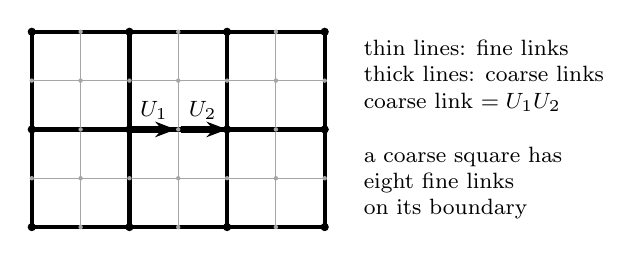
\begin{tikzpicture}[scale=0.62]
\draw[gray!70,line width=0.4pt] (0,0) grid (6,4);
\draw[black,line width=1.5pt] (0,0) grid[step=2] (6,4);
\foreach \x in {0,...,6} \foreach \y in {0,...,4} \fill[gray!70] (\x,\y) circle (1.3pt);
\foreach \x in {0,2,4,6} \foreach \y in {0,2,4} \fill (\x,\y) circle (2.4pt);
\draw[line width=2.6pt,-{Stealth[length=2.6mm]}] (2,2) -- (2.95,2);
\draw[line width=2.6pt,-{Stealth[length=2.6mm]}] (3.05,2) -- (4,2);
\node[above,font=\footnotesize] at (2.5,2) {$U_1$};
\node[above,font=\footnotesize] at (3.5,2) {$U_2$};
\node[right,font=\footnotesize,align=left] at (6.6,3.1) {thin lines: fine links\\ thick lines: coarse links\\ coarse link $=U_1U_2$};
\node[right,font=\footnotesize,align=left] at (6.6,0.9) {a coarse square has\\ eight fine links\\ on its boundary};
\end{tikzpicture}
\caption{A fine lattice and the coarse lattice of twice the mesh, in one spatial plane. The coarse field
keeps the product of the two fine links under each coarse link and forgets the rest.}\label{f:grid}
\end{figure}

Suppose three things.
\begin{enumerate}
\item[(a)] The guess decays in time as on the coarse lattice.
\item[(b)] Every function, whatever its guess, loses within two time steps a fixed fraction of its detail,
except for detail carried by an exceptional set of coarse fields.
\item[(c)] The dynamics seldom returns to that exceptional set.
\end{enumerate}
Then every function on the fine lattice decays almost as fast as the guesses do, up to two losses, which must
both be small: the return to
the exceptional set, and a factor that is close to one when the detail is lost in few steps compared with
the time considered. Theorem~\ref{t:inh} makes this precise.

The exceptions are allowed for a reason. A natural way to prove~(b) goes through local updates of the fine
links, and in our trials that route meets slow directions on selected coarse fields (Appendix~\ref{s:local}).
This is motivation only: the trials are statistical evidence about the particular functions tried, and
certify nothing about all functions.

Where this stands: Theorem~\ref{t:ret} proves a bound of the kind~(c) for $\SU(2)$, for exceptional sets
built from narrow neighbourhoods of one group element (we call them gates); it is not shown that~(b) can
hold with such sets. Statements (b) and~(a)
are open (Hypotheses~\ref{h:mix} and~\ref{h:coarse}). Chaining the refinement steps needs, in addition, a
bound on the accumulated losses, which is also open (Hypothesis~\ref{h:budget}).

\subsection{Main results}
\begin{theorem}[Spectral criterion]\label{t:crit}
Let $H\ge0$ be a self-adjoint operator on a Hilbert space $\cH$, let $\tau>0$, and let $D\subset\cH$ have dense
linear span. For $v\in\cH$ and $n\ge0$ put
\[
d_{v,n}=\big\langle v,\,e^{-n\tau H}\big(I-e^{-\tau H}\big)v\big\rangle\ \ge0 .
\]
Let $0<r<1$ and $\Delta=-\tau^{-1}\log r$. The following are equivalent.
\begin{enumerate}
\item $H$ has no spectrum in $(0,\Delta)$.
\item $\limsup_{n\to\infty}d_{v,n}^{1/n}\le r$ for every $v\in D$.
\end{enumerate}
\end{theorem}

Only the rate $r$ is common in (2); constants and the onset of the decay may depend on $v$. The criterion is
satisfied trivially when $H=0$, so by itself it says nothing about whether there is any positive energy; the
problem of~\cite{JW} also requires the mass to be finite.

\begin{theorem}[Refinement with an exceptional set]\label{t:inh}
Let $A$ be a self-adjoint operator on a non-zero Hilbert space $\mathcal K$ with $0\le A\le I$. Let $P$ be an
orthogonal projection, $Q=I-P$, and let $B$ be an orthogonal projection with range inside the range of $Q$;
put $G=Q-B$. Let $m\ge j\ge1$ be integers, $\gamma>0$, $\kappa\ge0$ and $b\in\R$, and suppose
\begin{equation}\label{e:hyp}
\langle f,(I-A^{2})f\rangle\ge\gamma\|Gf\|^2\ \ (f\in\mathcal K),\qquad
\|BA^{j}B\|\le\kappa,\qquad \|PA^{m}P\|\le1-b .
\end{equation}
Then
\begin{equation}\label{e:inh}
1-\|A^m\|\ \ge\ \frac{(b-\kappa)_+}{1+2/(m\gamma)} .
\end{equation}
\end{theorem}

Here $(s)_+=\max\{s,0\}$. The space splits into a coarse part $P$, an exceptional part $B$ and a good part
$G$, and the three hypotheses are (b), (c) and (a) above, in that order:
\begin{itemize}
\item a function loses, within two steps, at least the fraction $\gamma$ of the squared norm of its good
part;
\item the exceptional part overlaps with itself after $j$ steps by at most $\kappa$;
\item the coarse part alone already has deficit $b$ after $m$ steps.
\end{itemize}
The third hypothesis only names the deficit $b$ of the coarse part; that $b$ is close to the deficit of the
coarse lattice, as~(a) supposes, is a separate statement (Hypothesis~\ref{h:coarse}).
The conclusion is that the whole space has deficit at least $b-\kappa$, divided by a factor that tends to $1$
when $m\gamma\to\infty$.

In the application $A$ is one step of a transfer semigroup. If $A=e^{-aH}$ with $H\ge0$ and mesh $a$, then
$A^m=e^{-tH}$ for $t=ma$, the left side of~\eqref{e:inh} is the \emph{deficit} $d=1-e^{-t\inf\sigma(H)}$ at
physical time $t$, and the denominator is $1+2a/(\gamma t)$. No logarithm of $A$ is needed, and $A$ may have
a kernel. In detail (terms are defined in Section~\ref{s:set}; symbols are listed in Table~\ref{tab:sym}),
$\mathcal K$ is the space of gauge-invariant functions of one time slice of the fine lattice with vacuum
expectation zero, $A$ is one step of the transfer semigroup in the vacuum representation, $P$ is the
conditional expectation given the coarse links, and $B$ is the part of $Q$ supported on an exceptional set of
coarse fields. A physical time $t$ corresponds to $m=t/a$ steps, so $m$ doubles when the mesh is halved. On
this space $1-\|A^m\|>0$ says that this lattice has a gap, with $\Delta=-t^{-1}\log\|A^m\|$; at one fixed
lattice that is elementary (Section~\ref{s:not}), and the question is what survives refinement.

\begin{theorem}[Return to a coarse plaquette gate]\label{t:ret}
Consider the Wilson measure with weight $\exp\big(\beta\sum_p\tfrac12\Tr U_p\big)$, $\beta\ge0$, for the gauge
group $\SU(2)$ on a periodic lattice with even spatial side $N\ge6$ and $T\ge2$ time slices. Fix a spatial
plaquette of side two (a coarse plaquette) and $0\le\theta\le\pi$. Let $x$ and $y$ be the spatial links of
two time slices that are distinct modulo $T$. For the spatial links of a time slice let $\Gamma_\theta$ be the
event that the holonomy around that plaquette (the ordered product of its eight fine links) lies within round
distance $\theta$ of $-I$ (the angle between the two as points of $S^3$); we call $\Gamma_\theta$ a
\emph{gate}. Then for every complex square-integrable function $g$ of a slice, with
$h=\mathbf 1_{\Gamma_\theta}g$,
\begin{equation}\label{e:ret}
\big|\E\big[\overline{h(x)}\,h(y)\big]\big|\ \le\ p_{6\beta}(\theta)\,\E\big[|h(x)|^2\big],
\qquad
p_k(\theta)=\frac{\int_0^\theta\sin^2\!\varphi\,e^{k(\cos\varphi-1)}\,d\varphi}{\int_0^\pi\sin^2\!\varphi\,e^{k(\cos\varphi-1)}\,d\varphi},
\end{equation}
and $p_k(\theta)\le\min\{1,\ \tfrac{\pi^2\sqrt e}{4}(1+k)^{3/2}\theta^3\}$.
\end{theorem}

In words: whatever the field is at one time, the conditional probability that the chosen plaquette is within
$\theta$ of $-I$ at another time is at most $p_{6\beta}(\theta)$, which is of order $\theta^3$. Three remarks
on its reach.
\begin{itemize}
\item The order $\theta^3$ is for fixed $\beta$; the bound is small only for $\theta$ well below
$(6\beta)^{-1/2}$.
\item The bound does not depend on the spatial volume, on the time separation or on the rest of the field.
\item The gate is centred at $-I$ because the smallest local quotients we measured are on a background with
three plaquettes at $-I$ (Appendix~\ref{s:local}: two backgrounds, one lattice, one coupling); this is a
choice suggested by those trials, not a result.
\end{itemize}
Corollary~\ref{c:vac} carries the bound to the vacuum on an infinite time axis, where it becomes the second
inequality of~\eqref{e:hyp}.

Two further results are proved. Proposition~\ref{p:three} in Section~\ref{s:crit} is a form of the criterion
that uses a single time separation. Proposition~\ref{p:haar} in Appendix~\ref{s:haar} gives an explicit lower
bound for the conditional variance of a single link; it bounds one term of the auxiliary statement of
Section~\ref{s:arch} and is not an input of Theorem~\ref{t:inh}.

\subsection{What is not claimed}\label{s:not}
\begin{enumerate}
\item No mass gap is proved in infinite volume or in the continuum, and no lower bound uniform along a
refinement, for any gauge group. (At a fixed finite lattice a gap exists for elementary reasons and is not
the issue.)
\item No continuum theory is constructed. We have not examined the construction~\cite{OAI} beyond two declarations
(Section~\ref{s:ext}); we rely on its assessment~\cite{YMG} for what it does and does not contain, and we have not shown that any object of this
paper belongs to it (Section~\ref{s:ext}).
\item Theorem~\ref{t:inh} is conditional. Of its three hypotheses the second is proved for $\SU(2)$
(Corollary~\ref{c:vac}). The first and the third are open (Hypotheses~\ref{h:mix} and~\ref{h:coarse}), and so
is the budget that chaining the steps needs (Hypothesis~\ref{h:budget}); none is proved on any trajectory of
matched couplings. Even with all of them the conclusion concerns a fixed physical box and is not a gap in
infinite volume.
\item Theorem~\ref{t:ret} and all measurements are for $\SU(2)$. The gate around $-I$ and the constant $p_{6\beta}(\theta)$
are special to it; that constant is the largest value over the conditional laws that one link can have, and
is not shown to be attained on any Wilson background. For other groups only a cruder return bound is available (Remark~\ref{r:ret}(d)), and
whether a useful exceptional set exists is open.
\item The refinement step is stated on the centred gauge-invariant functions of a slice. Related hypotheses
in the working notes (Supplement~S9) are stated on the smaller space that is also neutral under the centre of the group. A
result on one of these spaces is not a result on the other, and which space matters depends on the domain of
the continuum theory one compares with.
\item The measurements of Section~\ref{s:evid} are Monte Carlo estimates on lattices of side $5$ to $10$,
one coupling each, with statistical errors. The exact value of a trial function limits a constant from one
side; an estimate of it is not a bound. The estimates are statistical evidence about the functions tried; they do
not certify an inequality over all functions or its limit, and none is
used in a proof.
\end{enumerate}

How the results were obtained, which parts are machine-checked, and the fact that the paper has not been
peer reviewed are set out in Section~\ref{s:disc}.

\subsection{Organisation}
Section~\ref{s:set} fixes the setting and the notation. Section~\ref{s:arch} states the open hypotheses and
shows, in Figure~\ref{f:arch}, how the proved and the open statements fit together. The proofs follow in
Sections~\ref{s:crit} to~\ref{s:ret}. Section~\ref{s:evid} summarises the measurements, Section~\ref{s:ext}
relates the paper to the external construction, and Section~\ref{s:rem} lists what remains. The appendices
hold the measurements in full, the one-link covariance bound, the machine-checked parts and the catalogue of
supplementary material, and a check of the outline in the free theory. A reader who wants only the mathematics can read Sections~\ref{s:set}
to~\ref{s:ret}; a reader who wants only the state of the question can read this introduction,
Section~\ref{s:arch} and Section~\ref{s:rem}.

\section{Setting and notation}\label{s:set}
\emph{Lattice.} A periodic lattice has $N$ sites in each of three spatial directions and $T$ time slices.
A \emph{link} joins two neighbouring sites and a \emph{plaquette} is an elementary square of four links.
Links carry elements of $\SU(2)$, identified with unit quaternions and with the unit sphere $S^3\subset\R^4$;
$\tfrac12\Tr(U^{-1}V)$ is the inner product of $U$ and $V$ in $\R^4$, and the round distance
$\operatorname{dist}(U,V)\in[0,\pi]$ is the angle between them. The Wilson measure has density proportional
to $\exp(\beta\sum_p\tfrac12\Tr U_p)$ with respect to Haar measure on the links, the sum over plaquettes $p$ and $\beta\ge0$ the coupling
(large $\beta$ is weak coupling),
with $U_p$ the ordered product of the four links of $p$. A \emph{slice} is the collection of spatial links at
one time.

\emph{Transfer operator.} Fix a finite spatial lattice and $\beta>0$. On $L^2$ of the slice configurations
with Haar measure let $\mathsf T_0$ be the transfer operator in temporal gauge~\cite{Lu77,OS78} and $\Pi$ the
orthogonal projection onto the gauge-invariant functions (the average over gauge transformations at the
sites of the slice). The operator of the periodic lattice with its time-like links integrated is
$\mathsf L=\mathsf T_0\Pi=\Pi\mathsf T_0$ (Lemma~\ref{l:trace}). It is self-adjoint and positive semidefinite, it
vanishes on the functions with $\Pi f=0$, and on the gauge-invariant functions it is positive and injective.
$\Lambda_0$ is its largest eigenvalue and $\Omega>0$ the corresponding eigenfunction, which is gauge invariant.
The \emph{vacuum representation} is $L^2(\Omega^2\,d\mathrm{Haar})$ with
$S_1f=\Lambda_0^{-1}\Omega^{-1}\mathsf L(\Omega f)$, a self-adjoint contraction with $0\le S_1\le I$ and $S_11=1$,
and $S_n=S_1^n$. Time is counted in lattice steps; one step is the mesh $a$ in physical units. On the
gauge-invariant functions $S_1$ is injective, so there $S_n=e^{-naH}$ with $H=-a^{-1}\log S_1\ge0$ the Hamiltonian in physical
units. We do not need $H$: Theorem~\ref{t:inh} is applied with $A=S_1$ restricted to the
gauge-invariant functions that are \emph{centred}, that is, have vacuum expectation zero.

\emph{Coarse links.} For even $N$, the coarse links of a slice are the products of two consecutive fine
spatial links between sites with even coordinates. A function of a slice is \emph{coarse-measurable} if it
depends on the coarse links only. A \emph{coarse plaquette} is a spatial square of side two with even corners;
its holonomy is the product of its eight fine links. A \emph{background} is a configuration of the coarse
links of a slice.

\emph{Refinement sequence.} A \emph{fixed physical box} is a sequence of lattices of mesh $a_i=a_0/2^i$ and
spatial side $N_i=2^iN_0$, so that the side $N_ia_i$ in physical units does not change. Couplings $\beta_i$ are
\emph{matched} if a chosen renormalised coupling at the scale of the box has the same value on every lattice
of the sequence; such a sequence of lattices and couplings is a \emph{trajectory of matched couplings}.

\emph{Local updates.} A \emph{colour} is one of $24$ classes of pairs of fine links inside coarse cells, such
that the pairs of one class can be resampled together from their conditional law given all other links,
leaving the coarse links unchanged; the classes are those of the sampling program (Supplement~S1; the supplement is catalogued in
Appendix~\ref{app:supp}). For a function
$F$ of a slice, on a fixed coarse background, $\mathcal J(F)$ is the average over the $24$ colours of the
expected conditional variance of $F$ under the resampling of that colour, and $\mathcal V(F)$ is the
conditional variance of $F$ given the coarse links. We call $\mathcal J(F)/\mathcal V(F)$ the \emph{local
quotient} of $F$. It measures relaxation under these artificial updates, not under the transfer operator.

\begin{table}[ht]
\centering\small
\begin{tabular}{@{}lll@{}}
\toprule
Symbol & Meaning & Where \\
\midrule
$H$ & Hamiltonian & Thm~\ref{t:crit} \\
$A$, $S_n=S_1^n$ & one transfer step; powers of the vacuum transfer step & Thm~\ref{t:inh}, \S\ref{s:set} \\
$d_{v,n}$ & differences of the correlation of $v$ with itself & Thm~\ref{t:crit} \\
$P$, $Q$, $B$, $G$ & coarse projection; its complement; exceptional and good parts & Thm~\ref{t:inh} \\
$a$, $t$, $m$, $j$ & fine mesh; physical time; $m=t/a$ steps; a lag of $j\le m$ steps & Thm~\ref{t:inh} \\
$\gamma$, $\kappa$, $b$, $d$ & mixing rate; return weight; deficit of the coarse part; deficit $1-\|A^m\|$ & \eqref{e:hyp}, \eqref{e:inh} \\
$N$, $T$, $\beta$ & spatial side; time slices; bare coupling & Section~\ref{s:set} \\
$\mathsf L$, $\Omega$ & transfer operator at fixed spatial lattice; its vacuum & Section~\ref{s:set} \\
$\Gamma_\theta$, $p_k(\theta)$ & gate around $-I$; cap probability at tilt $k$ & Thm~\ref{t:ret} \\
$\chi$ & multiplication by the indicator of the gate & Cor.~\ref{c:vac} \\
$K_i$, $M_i$ & loss factor of the $i$th refinement; product $K_1\cdots K_i$ & Cor.~\ref{c:acc} \\
$\varepsilon_i$ & loss allowed in the comparison with the coarser lattice & Hyp.~\ref{h:coarse} \\
$\varrho(c)$ & maximal correlation of consecutive slices given the coarse field $c$ & Prop.~\ref{p:pred} \\
$R=I_2/I_1$ & mean of $u\cdot v$ under the tilted law on $S^3$ & Prop.~\ref{p:haar} \\
$\mathcal J$, $\mathcal V$ & loss under local updates; conditional variance & Section~\ref{s:set} \\
$\mathsf R(f)$ & two-time quotient $1-C_f(\text{lag})/C_f(0)$ & Appendix~\ref{s:cross} \\
\bottomrule
\end{tabular}
\caption{Principal symbols.}\label{tab:sym}
\end{table}

\section{Outline and the open hypotheses}\label{s:arch}
Figure~\ref{f:arch} is the outline. Read it from the top. Theorem~\ref{t:inh} treats one halving of the mesh and
has three inputs: the return bound, which is Theorem~\ref{t:ret} with Corollary~\ref{c:vac}; decay off the
gates (Hypothesis~\ref{h:mix}); and comparison with the coarse lattice (Hypothesis~\ref{h:coarse}).
Corollary~\ref{c:acc} chains the halvings and needs one more input, the budget (Hypothesis~\ref{h:budget}). The
three hypotheses are open, so every box on the path from Theorem~\ref{t:inh} down to the mass gap is open.
Theorem~\ref{t:crit} enters only at the bottom: it says what would have to be checked in a continuum theory.

This would be one sufficient route to a gap in a box, if the three hypotheses held. A direct estimate of the differences $d_{v,n}$ in the
continuum theory would meet the criterion of Theorem~\ref{t:crit} without it.

\begin{figure}[ht]
\centering
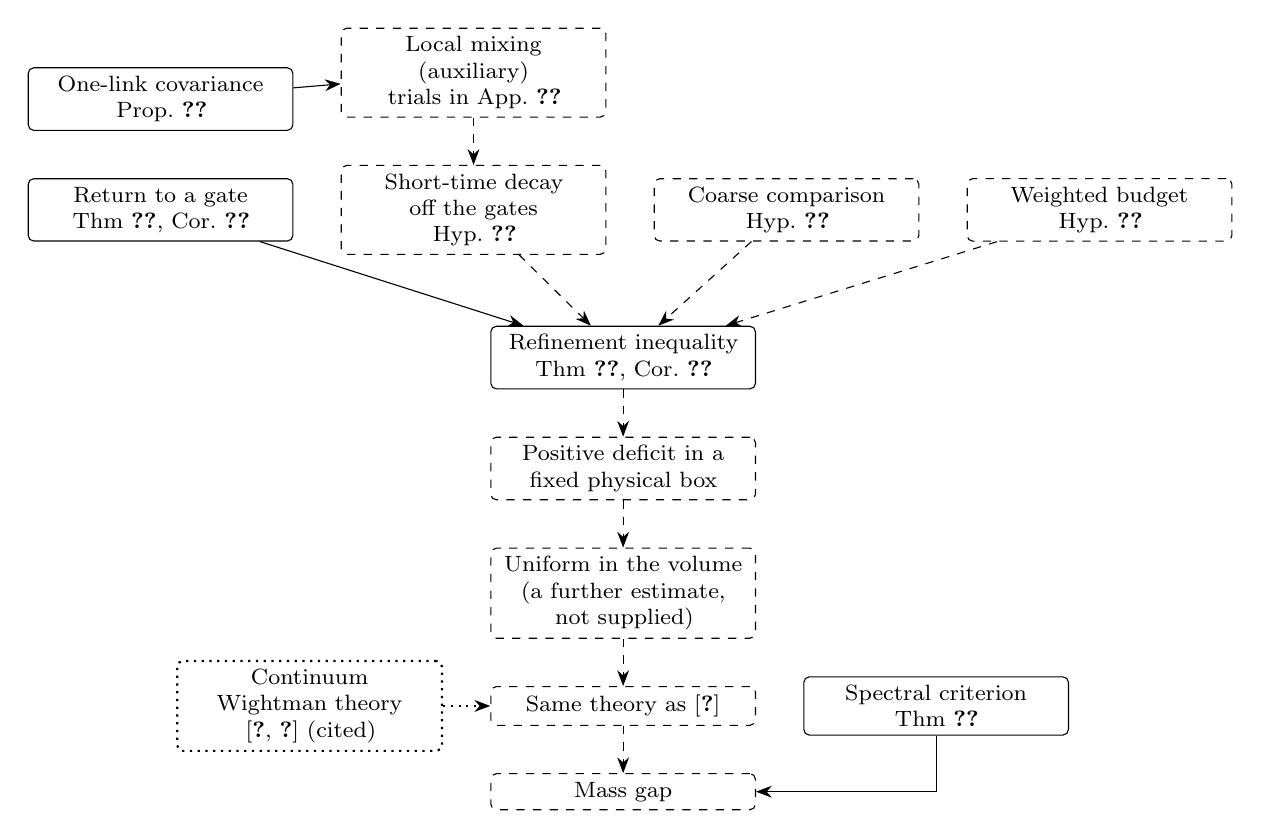
\begin{tikzpicture}[node distance=6mm and 6mm,
 prov/.style={draw,rounded corners=2pt,align=center,font=\footnotesize,inner sep=3pt,text width=31.5mm},
 open/.style={prov,dashed},
 ext/.style={prov,dotted,thick},
 >={Stealth[length=2mm]}]
\node[prov] (ret) {Return to a gate\\ Thm~\ref{t:ret}, Cor.~\ref{c:vac}};
\node[open,right=of ret] (mix) {Short-time decay\\ off the gates\\ Hyp.~\ref{h:mix}};
\node[open,right=of mix] (coarse) {Coarse comparison\\ Hyp.~\ref{h:coarse}};
\node[open,right=of coarse] (budget) {Weighted budget\\ Hyp.~\ref{h:budget}};
\node[prov,below=9mm of mix,xshift=19mm] (inh) {Refinement inequality\\ Thm~\ref{t:inh}, Cor.~\ref{c:acc}};
\node[open,above=of mix] (aux) {Local mixing\\ (auxiliary)\\ trials in App.~\ref{s:local}};
\node[prov,above=of ret] (haar) {One-link covariance\\ Prop.~\ref{p:haar}};
\node[open,below=of inh] (box) {Positive deficit in a\\ fixed physical box};
\node[open,below=of box] (vol) {Uniform in the volume\\ (a further estimate,\\ not supplied)};
\node[open,below=of vol] (same) {Same theory as~\cite{OAI}};
\node[ext,left=of same] (ext) {Continuum\\ Wightman theory\\ \cite{OAI,YMG} (cited)};
\node[prov,right=of same] (crit) {Spectral criterion\\ Thm~\ref{t:crit}};
\node[open,below=of same] (gap) {Mass gap};
\draw[->] (ret) -- (inh);
\draw[->,dashed] (mix) -- (inh);
\draw[->,dashed] (coarse) -- (inh);
\draw[->,dashed] (budget) -- (inh);
\draw[->,dashed] (aux) -- (mix);
\draw[->] (haar) -- (aux);
\draw[->,dashed] (inh) -- (box);
\draw[->,dashed] (box) -- (vol);
\draw[->,dashed] (vol) -- (same);
\draw[->,dashed] (same) -- (gap);
\draw[->,dotted,thick] (ext) -- (same);
\draw[->] (crit) |- (gap);
\end{tikzpicture}
\caption{Outline. Solid boxes are proved in this paper; Corollary~\ref{c:vac} rests on Lemma~\ref{l:trace}.
Dashed boxes are open. The dotted box is cited. An arrow from $X$ to $Y$
means that $X$ is an input of $Y$; it is solid when $X$ is proved and dashed when $X$ is open.
Hypothesis~\ref{h:budget} enters through Corollary~\ref{c:acc}.}\label{f:arch}
\end{figure}

\begin{hypothesis}[Short-time decay off the gates; open]\label{h:mix}
For a sequence of lattices of mesh $a_i=a_0/2^i$ in a fixed physical box, with one-step operators $A_i$ on the
centred gauge-invariant functions, exceptional projections $B_i$ built from gates as in Corollary~\ref{c:vac},
$Q_i=I-P_i$ the complement of the coarse projection $P_i$ and $G_i=Q_i-B_i$, there are $\gamma_i>0$ with $\langle f,(I-A_i^2)f\rangle\ge\gamma_i\|G_if\|^2$ for all $f$, and
$\sum_ia_i/\gamma_i<\infty$.
\end{hypothesis}

\begin{hypothesis}[Coarse comparison; open]\label{h:coarse}
Fix a physical time $t$ that is a multiple of $a_0$, and let $m_i=t/a_i$. For $i\ge1$ let $P_i$ be the conditional
expectation given the coarse links (of mesh $2a_i$) of the lattice of mesh $a_i$, on the centred gauge-invariant functions. With $d_{i-1}=1-\|A_{i-1}^{m_{i-1}}\|$
the deficit of the lattice of mesh $2a_i$ at matched coupling, $\|P_iA_i^{m_i}P_i\|\le1-b_i$ with
$b_i\ge d_{i-1}-\varepsilon_i$, for real numbers $b_i$ and $\varepsilon_i\ge0$ that are constrained only through
Hypothesis~\ref{h:budget}.
\end{hypothesis}

\begin{hypothesis}[Weighted budget; open]\label{h:budget}
With $\gamma_i$ as in Hypothesis~\ref{h:mix}, $K_i=1+2/(m_i\gamma_i)=1+2a_i/(\gamma_it)$, $M_0=1$, $M_i=K_1\cdots K_i$, $\kappa_i\ge0$ such
that $\|B_iA_i^{j_i}B_i\|\le\kappa_i$ for some integer $1\le j_i\le m_i$, and $\varepsilon_i$ as in
Hypothesis~\ref{h:coarse}, the series below converges and
\[
\sum_{i=1}^\infty M_{i-1}(\varepsilon_i+\kappa_i)\ <\ d_0 .
\]
\end{hypothesis}

At a fixed finite lattice each $A_i$ is compact and, on the centred functions, has norm below one (the eigenvalue
one of the full operator is simple and belongs to the constants; the largest eigenvalue on the centred
functions may be degenerate). So some $\gamma_i>0$ and some deficit exist, with no uniformity; and at strong coupling
there are estimates of this kind (working notes, Supplement~S8; not used here). What is
not proved is the three statements together, with the stated sums, on one trajectory of matched couplings
tending to weak coupling. If all held on one trajectory, Corollaries~\ref{c:acc} and~\ref{c:vac} would give a positive lower limit of the deficits in a
fixed physical box. Summability of the $\kappa_i$ and $\varepsilon_i$ alone would not: the budget is a
separate condition (Remark~\ref{r:budget}). Uniformity in the volume and the identification of the limit with
a continuum theory would remain.

\subsection{Two ways one might approach Hypothesis~\ref{h:mix}}
Hypothesis~\ref{h:mix} is about the transfer semigroup. One route to it uses the local updates of
Section~\ref{s:set}. A derivation in the working notes (Supplement~S8), not reproduced or checked here, bounds
$\langle f,(I-A^2)f\rangle$ from below by the expected loss of $f$ under those updates. Given that, it would
suffice to bound the local quotient $\mathcal J(F)/\mathcal V(F)$ from below for every function $F$ on every
background outside the gates. We call this the \emph{auxiliary local mixing statement}. It is stronger than
Hypothesis~\ref{h:mix}: a function that the local updates relax slowly may still decay quickly in time.

There is also a sufficient condition that involves only the physical time step. It asks how well the next
time slice predicts the fine detail of the present one when the coarse field of the present slice is known.

\begin{proposition}[Conditional prediction]\label{p:pred}
At a fixed lattice let $X$ and $Y$ be consecutive time slices of the stationary process with one-step operator
$A=S_1$, so that $(Af)(x)=\E[f(Y)\mid X=x]$, and let $C$ be the coarse field of $X$. For a coarse field $c$ let
$\varrho(c)$ be the maximal correlation of $X$ and $Y$ given $C=c$, that is, the supremum of the absolute value of the correlation
of $f(X)$ and $g(Y)$ under the conditional law, over square-integrable complex $f$ and $g$ (centred under
that law and of non-zero variance there; $\varrho(c)=0$ if there are none). Let $\mathcal G$ be a
measurable set of coarse fields, invariant under gauge transformations of the coarse lattice, and $G=\mathbf 1_{\mathcal G}(C)\,(I-P)$. If $\varrho(c)^2\le1-\gamma$ for
almost every $c\in\mathcal G$, then $\langle f,(I-A^2)f\rangle\ge\gamma\|Gf\|^2$ for every $f$.
\end{proposition}
\begin{proof}
The configuration spaces are compact and metrisable, so regular conditional laws exist and $\varrho$ is
measurable (a supremum over a countable dense family). The pair $(X,Y)$ is exchangeable because $A$ is self-adjoint, so $\|Af\|^2=\E\,|\E[f(X)\mid Y]|^2$ and
$\langle f,(I-A^2)f\rangle=\E\operatorname{Var}(f(X)\mid Y)$. Conditioning on more cannot increase the expected
conditional variance, so this is at least $\E\operatorname{Var}(f(X)\mid Y,C)$. Under the conditional law given
$C=c$, the expected conditional variance of $f(X)$ given $Y$ equals its variance minus the variance of its
best prediction from $Y$, which is at least $(1-\varrho(c)^2)\operatorname{Var}(f(X)\mid C=c)$. Integrating
over $c\in\mathcal G$ and discarding the rest gives
$\gamma\,\E[\mathbf 1_{\mathcal G}(C)\operatorname{Var}(f(X)\mid C)]=\gamma\|Gf\|^2$.
\end{proof}

So Hypothesis~\ref{h:mix} would follow from a bound on the conditional maximal correlation outside the gates,
with $\sum_ia_i/\gamma_i<\infty$. We have no such bound for the Wilson measure at weak coupling; the
proposition replaces one open estimate by another and proves nothing about the theory. It does say what the
measurement of Appendix~\ref{s:time} is a trial for: a correlation between a function of one slice and a
function of the next, given the coarse field of the first, is, in the population, a lower value for the conditional maximal
correlation on that coarse field. Three reservations apply. Here $g$ must be a function of the next slice
alone. The measurement is on a periodic lattice with one slice frozen, so the quantity concerned is the
analogue $\varrho_T(c)$ for period $T$, not the vacuum quantity $\varrho(c)$ of the proposition, and we have
no estimate of their difference. And a Monte Carlo estimate at one coarse field is neither a certified bound
there nor a statement about almost every field. A small mutual information of $X$ and $Y$ given $C$ is not enough, since $\varrho$ is a supremum over
normalised functions, including those concentrated on rare configurations.

\begin{remark}[How weak the mixing rate may be]\label{r:rate}
Hypothesis~\ref{h:mix} asks only for $\sum_ia_i/\gamma_i<\infty$. Suppose that along the trajectory the
couplings grow at most logarithmically in the mesh, $\beta_i\le s\log(1/a_i)+\text{const}$. Then a rate
$\gamma_i\ge Ce^{-c\beta_i}$ with $c<1/s$ is enough, because $a_i/\gamma_i$ is then at most a constant times
$a_i^{1-cs}$, which is summable over dyadic meshes. Logarithmic growth is what asymptotic freedom predicts:
at one loop $s=11/(3\pi^2)\approx0.37$ for $\SU(2)$, and the matched couplings of
Appendix~\ref{app:meas} give $s\approx0.43$ between sides $5$ and $10$. We do not prove the growth
condition; for the trajectory of the external construction it is reported in its assessment
(Section~\ref{s:ext}). The remark says that the difficulty of Hypothesis~\ref{h:mix} is not the size of the rate, for
which a bound exponentially small in $\beta$ would do if the growth condition holds, but its uniformity in
the volume and in the coarse field. (The measured slope is an illustration, not a bound on the trajectory;
and any $\gamma_i$ with $\sum_ia_i/\gamma_i<\infty$ would do, for instance $\gamma_i=a_i\,i^{1+\delta}$.)
\end{remark}

\begin{remark}[An exact form and a sufficient form of Hypothesis~\ref{h:mix}]\label{r:forms}
\leavevmode
\begin{enumerate}
\item[(a)] \emph{Exact.} At a fixed lattice $\|A\|<1$ on the centred functions, so $I-A^2$ is invertible, and
for a projection $G\ne0$ the best constant in $I-A^2\ge\gamma G$ is
\[
\gamma_{\mathrm{opt}}=\big\|G(I-A^2)^{-1}G\big\|^{-1},\qquad
\gamma_{\mathrm{opt}}^{-1}=\sup_{h\in\operatorname{ran}G,\ \|h\|=1}\ \sum_{n\ge0}\langle h,A^{2n}h\rangle .
\]
Indeed the inequality is equivalent to $I\ge\gamma(I-A^2)^{-1/2}G(I-A^2)^{-1/2}$, and the operator on the
right has the norm of $G(I-A^2)^{-1}G$. So Hypothesis~\ref{h:mix} is the statement that
$\sum_ia_i\|G_i(I-A_i^2)^{-1}G_i\|<\infty$: the fine detail off the gates must not retain too much
correlation summed over time. It does not ask for more. In terms of the Hamiltonian, $A_i=e^{-a_iH_i}$ on the
centred gauge-invariant functions and $1/x\le1/(1-e^{-x})\le1+1/x$ give
$\tfrac12\|GH^{-1}G\|\le a\,\|G(I-A^2)^{-1}G\|\le a+\tfrac12\|GH^{-1}G\|$. Since the meshes are summable,
Hypothesis~\ref{h:mix} holds for some choice of the $\gamma_i$ if and only if
$\sum_i\|G_iH_i^{-1}G_i\|<\infty$.
\item[(b)] \emph{Sufficient.} Work in temporal gauge, before the gauge projection: let $Y$ given $X=x$ have
density proportional to $\mathsf C(x,y)\phi(y)=\exp(\beta\sum_ex_e\cdot y_e)\phi(y)$, links being unit vectors in
$\R^4$ and $\phi=W\Omega$ as in Remark~\ref{r:doob} below. The joint density of $(X,Y)$ is
$\phi(x)\mathsf C(x,y)\phi(y)/\Lambda_0$, which is symmetric, and this process has the same action on
gauge-invariant functions as the transfer step, so Proposition~\ref{p:pred} may be applied to it and its
conclusion restricted to those functions. For a function $g$
of $Y$ and $h(x)=\E[g(Y)\mid X=x]$, the derivative of $h$ along a tangent vector $v$ is
$\beta\Cov(g(Y),\sum_ev_e\cdot Y_e\mid X=x)$. Suppose that on a coarse field $c$ the covariance of $Y$ given
$X=x$ has operator norm at most $L_c$, and that the law of $X$ given $C=c$ satisfies a Poincar\'e inequality
$\operatorname{Var}(h)\le P_c\,\E|\nabla h|^2$ with the gradient along the fibre (the variations of the
links that keep the coarse links fixed). Then
$\operatorname{Var}(h(X)\mid C=c)\le\beta^2P_cL_c\,\E[\operatorname{Var}(g(Y)\mid X)\mid C=c]$, and by the
law of total variance
\[
\varrho(c)^2\le\frac{\beta^2P_cL_c}{1+\beta^2P_cL_c},\qquad\text{so that}\qquad
\gamma\ge\frac1{1+\beta^2\operatorname*{ess\,sup}_{c\in\mathcal G}P_cL_c}
\]
in Proposition~\ref{p:pred}. With Remark~\ref{r:rate}, bounds $P_c\le C_1e^{p\beta}$ and
$L_c\le C_2e^{q\beta}$, uniform in the volume, would suffice when $p+q<1/s$. Since $h$ is gauge invariant when $g$ is, the Poincar\'e
inequality is needed only for gauge-invariant functions on the fibre. Neither bound is known for the Wilson
measure at weak coupling. In the free theory the reduction loses little: there $\beta P_c$ tends to $0.617$
and $\beta L_c$ to $1$ as the side grows, which gives $\gamma\ge0.618$ where the true value is $0.675$
(Appendix~\ref{app:free}, Supplement~S11).
\end{enumerate}
Both forms were proposed by an OpenAI GPT model used as reviewer.
\end{remark}

\section{The spectral criterion}\label{s:crit}
The proof is the spectral theorem and one observation: a positive measure with mass just above zero energy
cannot hide it, because the differences $d_{v,n}$ are integrals of a non-negative function.

\begin{proof}[Proof of Theorem~\ref{t:crit}]
Let $E$ be the spectral measure of $H$ and $\mu_v(\cdot)=\langle v,E(\cdot)v\rangle$, a finite positive measure
on $[0,\infty)$. Then $d_{v,n}=\int_{[0,\infty)}e^{-n\tau s}(1-e^{-\tau s})\,d\mu_v(s)$; the integrand is
non-negative and vanishes at $s=0$.

(1)$\Rightarrow$(2). If $\mu_v$ gives no mass to $(0,\Delta)$ then $d_{v,n}\le e^{-n\tau\Delta}\|v\|^2=r^n\|v\|^2$.

(2)$\Rightarrow$(1). Let $v\in D$ and suppose $\mu_v((0,\Delta))>0$. Then there are $0<\alpha<\omega<\Delta$ with
$\mu_v([\alpha,\omega])>0$, and $d_{v,n}\ge e^{-n\tau\omega}(1-e^{-\tau\alpha})\mu_v([\alpha,\omega])$, so
$\limsup d_{v,n}^{1/n}\ge e^{-\tau\omega}>r$, a contradiction. Hence $E((0,\Delta))v=0$ for every $v\in D$.
The projection $E((0,\Delta))$ is bounded and vanishes on a set with dense span, so it is zero.
\end{proof}

\begin{remark}\label{r:crit}
\leavevmode
\begin{enumerate}
\item[(a)] The differences matter. Under (1), $|\langle v,e^{-n\tau H}(I-E_0)w\rangle|\le r^n\|v\|\,\|w\|$ with $E_0$ the
projection onto the kernel of $H$; the matrix elements $\langle v,e^{-n\tau H}w\rangle$ themselves need not decay,
since the vacuum contributes a constant.
\item[(b)] A polynomial bound on the low-energy weight,
$\mu_v((0,s])\le Cs^\nu$, does not give (2) for any $r<1$: a measure with density $s^{\nu-1}$ near $0$
satisfies it, and its differences $d_{v,n}$ decay only like a power of $n$.
\item[(c)] In a theory with several pure phases the criterion
may be applied in one component; a gap there says nothing about the others.
\item[(d)] The criterion is on the
diagonal, for single vectors, and positivity is what excludes cancellation; a test on finitely many vectors
can refute a proposed rate; it establishes a gap only if those vectors are known to span a dense subspace or, more generally, to
generate a dense subspace under bounded functions of $H$.
\end{enumerate}
\end{remark}

\begin{proposition}[A test at one time separation]\label{p:three}
With $H$ and $\tau$ as in Theorem~\ref{t:crit}, let $S=e^{-\tau H}$, $0<r<1$ and $\Delta=-\tau^{-1}\log r$, and let
$D_0\subset\cH$ be a dense linear subspace. Then $H$ has no spectrum in $(0,\Delta)$ if and only if
\[
(1+r)\langle v,Sv\rangle-\langle v,S^2v\rangle\ \le\ r\,\langle v,v\rangle\qquad\text{for all }v\in D_0 .
\]
\end{proposition}
\begin{proof}
The inequality says that the bounded self-adjoint operator $(rI-S)(I-S)$ is non-negative on $D_0$, hence on
$\cH$ by density. By the spectral theorem this holds exactly when $(r-x)(1-x)\ge0$ on the spectrum of $S$,
that is, when $S$ has no spectrum in $(r,1)$.
\end{proof}

\begin{remark}\label{r:three}
Here the test must hold on a linear subspace, not just on a spanning set: for $S=\operatorname{diag}(0.95,0.3)$
and $r=0.8$ the quadratic form $\langle v,(rI-S)(I-S)v\rangle$ equals $0.17125$ on each of $(1,\pm1)/\sqrt2$,
so the test is passed on a spanning set, and $-0.0075$ on $(1,0)$, where it fails; here $0.95\in(r,1)$. Theorem~\ref{t:crit} needs only a
spanning set but all large $n$; Proposition~\ref{p:three} needs three correlations at lags $0,\tau,2\tau$ but
every finite linear combination.
\end{remark}

\section{The refinement inequality}\label{s:inh}
The idea of the proof is to look at a vector that decays as slowly as anything can. Each hypothesis says that
such a vector has little weight in one of the three parts of the space, and the three weights add up to one.
We need one scalar inequality first.

\begin{lemma}\label{l:scal}
For $0\le x\le1$ and real $\rho\ge0$, $x(1-x^\rho)\le\rho(1-x)$.
\end{lemma}
\begin{proof}
For $x=0$ the left side is $0$. For $0<x\le1$, $1-x^\rho\le-\rho\log x$ because $1-e^{-s}\le s$, and
$-x\log x\le1-x$ because $\log(1/x)\le1/x-1$.
\end{proof}

\begin{proof}[Proof of Theorem~\ref{t:inh}]
Let $q=\|A\|$. If $q=0$ then $\|A^m\|=0$ and~\eqref{e:inh} holds because $b\le1$ by the third hypothesis and
$\kappa\ge0$. Let $q>0$, fix $0<q'<q$ and let $F=\mathbf 1_{[q',q]}(A)$. Since $A\ge0$ is self-adjoint, $q=\max\sigma(A)$, so $F\ne0$. Since $F$ commutes
with $A$ and $A^k(I-F)\ge0$, we have $A^k\ge A^kF\ge q'^kF$ for every integer $k\ge1$. Let $v$ be a unit
vector in the range of $F$.

\emph{Good part.} By the first hypothesis, $\gamma\|Gv\|^2\le\langle v,(I-A^2)v\rangle\le1-q'^2$.

\emph{Exceptional part.} $BA^jB\ge q'^jBFB$, so $\|FB\|^2=\|BFB\|\le\kappa/q'^j$, and
$\|Bv\|=\|BFv\|\le\|BF\|=\|FB\|$. Hence $\|Bv\|^2\le\kappa/q'^j$.

\emph{Coarse part.} In the same way $\|Pv\|^2\le\|FP\|^2=\|PFP\|\le\|PA^mP\|/q'^m\le(1-b)/q'^m$.

Since $B$ and $G$ are orthogonal projections with $B+G=Q$ and $BG=0$, $\|Qv\|^2=\|Gv\|^2+\|Bv\|^2$, and
$\|Pv\|^2=1-\|Qv\|^2$. Therefore
\[
1-\frac{1-b}{q'^m}\ \le\ \frac{1-q'^2}{\gamma}+\frac{\kappa}{q'^j} .
\]
Multiply by $x=q'^m\in(0,1]$ and use $q'^{m-j}\le1$: with $\rho=2/m$,
\[
b\ \le\ 1-x+\frac{x(1-x^{\rho})}{\gamma}+\kappa\ \le\ (1-x)\Big(1+\frac{\rho}{\gamma}\Big)+\kappa
\]
by Lemma~\ref{l:scal}. Let $q'\uparrow q$; since $A$ is self-adjoint, $\|A^m\|=q^m$, so
$1-\|A^m\|\ge(b-\kappa)/(1+\rho/\gamma)$. As $1-\|A^m\|\ge0$, \eqref{e:inh} follows.
\end{proof}

\begin{corollary}[Accumulation]\label{c:acc}
Let $d_0\ge0$ and, for $i=1,\dots,n$, let $K_i>0$ and $\kappa_i,\varepsilon_i,b_i,d_i\in\R$ satisfy
$d_i\ge(b_i-\kappa_i)/K_i$ and $b_i\ge d_{i-1}-\varepsilon_i$. With $M_0=1$ and $M_i=K_1\cdots K_i$,
\[
d_n\ \ge\ M_n^{-1}\Big(d_0-\sum_{i=1}^nM_{i-1}(\varepsilon_i+\kappa_i)\Big).
\]
For an infinite sequence with $K_i=1+2/(m_i\gamma_i)$, $m_i\ge1$ and $\gamma_i>0$, the products $M_n$ are
bounded if and only if $\sum_i1/(m_i\gamma_i)<\infty$; in that case, if moreover the series $\sum_iM_{i-1}(\varepsilon_i+\kappa_i)$ converges to a sum $s<d_0$
(Hypothesis~\ref{h:budget}), $\liminf_nd_n\ge(d_0-s)/\sup_nM_n>0$.
\end{corollary}
\begin{proof}
$M_id_i\ge M_{i-1}(b_i-\kappa_i)\ge M_{i-1}d_{i-1}-M_{i-1}(\varepsilon_i+\kappa_i)$; sum over $i$. The product of
factors $1+c_i$ with $c_i>0$ is bounded exactly when $\sum c_i<\infty$. Under Hypothesis~\ref{h:budget} the
partial sums of the budget converge to a limit $s<d_0$, so $\liminf_nd_n\ge(d_0-s)/\sup_nM_n>0$.
\end{proof}

\begin{remark}[The budget is needed]\label{r:budget}
Take $d_0=\tfrac12$, $K_i=1+2^{-i}$, $\varepsilon_i=0$, $b_i=d_{i-1}$, $\kappa_i=d_{i-1}/2$ and
$d_i=d_0/(2^iM_i)$. Every step satisfies the recurrence with equality, the $M_i$ are bounded and
$\sum\kappa_i<\infty$, yet $d_i\to0$. Here $\sum_iM_{i-1}\kappa_i=d_0$ exactly. The example is a recurrence,
not a lattice theory.
\end{remark}

\begin{remark}[Rarity alone is not enough]\label{r:reset}
The second hypothesis in~\eqref{e:hyp} is about return at a later time, not about the probability of the
exceptional set. An example: a process that, at rate $c>0$, replaces its state by an independent sample from
the stationary law, so that its semigroup is $e^{-ct}I+(1-e^{-ct})\,\E$ with $\E$ the stationary expectation.
Let the exceptional event be coarse-measurable, of arbitrarily small positive probability, and let it carry
a fine label that takes two values with equal probability independently of the coarse field. The function equal to $\pm1$ on the event according to the label, and $0$ elsewhere,
lies in the range of $B$ and is an eigenfunction with eigenvalue $e^{-ct}$. So the return weight at time $t$ is
$e^{-ct}$, whatever the probability of the event.
\end{remark}

\begin{remark}[A longer mixing lag]\label{r:lag}
If the first hypothesis in~\eqref{e:hyp} is replaced by $\langle f,(I-A^{2k})f\rangle\ge\gamma\|Gf\|^2$ for an
integer $k\ge1$, the same proof, with $\rho=2k/m$ in Lemma~\ref{l:scal}, gives~\eqref{e:inh} with denominator
$1+2k/(m\gamma)$. Along a refinement the products in Corollary~\ref{c:acc} then stay bounded when
$\sum_ik_ia_i/\gamma_i<\infty$, with $K_i=1+2k_i/(m_i\gamma_i)$ in Hypothesis~\ref{h:budget}. So the detail may take a number of steps that
grows, provided the physical times $k_ia_i$, each divided by $\gamma_i$, are summable.
\end{remark}

\begin{remark}[A second proof, machine-checked]\label{r:second}
The theorem can also be proved without a spectral projection. For a positive self-adjoint $A$ and every
$\eta>0$ there is a unit vector $w$ with $\|Aw-\|A\|w\|\le\eta$; then $\|A^nw-\|A\|^nw\|\le n\eta$ when
$\|A\|\le1$, and the three estimates of the proof above hold for $w$ up to errors of order $\eta$, the
exceptional and coarse parts by the Cauchy--Schwarz inequality for the positive form
$\langle\cdot,A^n\cdot\rangle$. Letting $\eta\to0$ gives~\eqref{e:inh}. This is the proof that is formalised
in Lean for all non-zero inner product spaces, real or complex (Appendix~\ref{s:lean}); it does not use
completeness.
\end{remark}

\section{Return to a coarse plaquette gate}\label{s:ret}
The return bound comes from a single link. Given all the other links, one link of the plaquette has an
explicit law on the sphere $S^3$, and for that law the probability of any cap is at most the probability of
the cap around the favoured point.

\begin{lemma}[Caps under a tilted law]\label{l:cap}
Let $u\in S^3$ have density $f_k(u)=e^{k\,u\cdot v}/Z(k)$ with respect to the uniform probability measure,
$k\ge0$, $v$ a unit vector; we call $k$ the \emph{tilt}. For every $c\in S^3$ and $0\le\theta\le\pi$, the probability of the cap
$\{u:\operatorname{dist}(u,c)\le\theta\}$ is at most that of the cap of the same radius centred at $v$, which
equals $p_k(\theta)$ and is non-decreasing in $k$.
\end{lemma}
\begin{proof}
The superlevel sets $\{f_k>s\}$ are caps centred at $v$. For a cap $\mathrm{Cap}_c$ centred at $c$ and the cap $\mathrm{Cap}_v$ of the
same radius centred at $v$, the uniform measure of $\{f_k>s\}\cap\mathrm{Cap}_c$ is at most the smaller of the measures of
the two sets, which is the measure of $\{f_k>s\}\cap\mathrm{Cap}_v$ because those two caps are concentric. Integrating
over $s$ gives $\int_{\mathrm{Cap}_c}f_k\le\int_{\mathrm{Cap}_v}f_k$. In the polar angle $\varphi$ from $v$ the uniform measure is
$\tfrac2\pi\sin^2\varphi\,d\varphi$, which gives the formula for $p_k$. Finally $\frac{d}{dk}\P_k(\mathrm{Cap}_v)=
\Cov_k(\mathbf 1_{\{\varphi\le\theta\}},\cos\varphi)\ge0$, because both are non-increasing functions of $\varphi$.
\end{proof}

\begin{proof}[Proof of Theorem~\ref{t:ret}]
Let $U$ be one of the eight fine links of the coarse plaquette in the slice of $y$. Condition on all other
links of the lattice; these include every link of the slice of $x$, because the two slices are distinct. The
holonomy is $XUY$ with $X,Y$ fixed, and $\operatorname{dist}(XUY,-I)=\operatorname{dist}(U,-X^{-1}Y^{-1})$ by
invariance of the round distance, so the event $y\in \Gamma_\theta$ is a cap of radius $\theta$ for $U$. The
conditional density of $U$ is proportional to $\exp(\beta\,\tfrac12\Tr(U\Sigma))$ with $\Sigma$ the sum of the
six staples of the link (a staple is the ordered product of the other three links of a plaquette through the
link; a link lies in six plaquettes), each a unit quaternion; writing $\Sigma=|\Sigma|\,v^{-1}$ (any unit $v$ if $\Sigma=0$) this is $e^{k\,u\cdot v}$ with
$k=\beta|\Sigma|\le6\beta$. By Lemma~\ref{l:cap}, $\P(y\in \Gamma_\theta\mid\text{all other links})\le
p_{6\beta}(\theta)$, and by the tower property $\P(y\in \Gamma_\theta\mid x)\le p_{6\beta}(\theta)$ almost surely.

The joint law of $(x,y)$ is invariant under exchanging the two slices: the reflection of the time coordinate
$s\mapsto s_x+s_y-s$ modulo $T$, where $s_x$ and $s_y$ are the times of the two slices, preserves the Wilson measure and swaps them. Hence
\begin{align*}
\big|\E[\overline{h(x)}h(y)]\big|&\le\tfrac12\E\big[\mathbf 1_{\Gamma_\theta}(x)\mathbf 1_{\Gamma_\theta}(y)(|g(x)|^2+|g(y)|^2)\big]\\
&=\E\big[|h(x)|^2\,\P(y\in \Gamma_\theta\mid x)\big]\ \le\ p_{6\beta}(\theta)\,\E|h(x)|^2 .
\end{align*}
For the envelope: the numerator of $p_k$ is at most $\theta^3/3$. On $0\le\varphi\le(1+k)^{-1/2}\le1$ we have
$\sin\varphi\ge2\varphi/\pi$ and $k(1-\cos\varphi)\le k\varphi^2/2\le\tfrac12$, so the denominator is at least
$\tfrac{4}{\pi^2}e^{-1/2}\cdot\tfrac13(1+k)^{-3/2}$.
\end{proof}

\subsection{Passage to the vacuum}
\begin{lemma}[Trace formula]\label{l:trace}
Fix a finite spatial lattice, $\beta>0$ and $T\ge2$. Let $W$ be multiplication by the square root of the
weight of the spatial plaquettes of a slice, $\mathsf C$ the operator with kernel
$\prod_e\exp\big(\beta\,\tfrac12\Tr(U_eV_e^{-1})\big)$, the product over the spatial links $e$ of the slice, and
$\mathsf T_0=W\mathsf CW$. Then $\mathsf L=\mathsf T_0\Pi=\Pi\mathsf T_0$ is a self-adjoint, positive semidefinite
integral operator with a continuous, strictly positive kernel, and for bounded functions
$f_0,\dots,f_{T-1}$ of a slice
\begin{equation}\label{e:trace}
\E_T\Big[\prod_{s}f_s(x_s)\Big]=\frac{\Tr\big(M_{f_0}\mathsf L\,M_{f_1}\mathsf L\cdots M_{f_{T-1}}\mathsf L\big)}{\Tr(\mathsf L^T)},
\end{equation}
where $\E_T$ is the expectation in the Wilson measure with $T$ time slices and $M_f$ is multiplication by
$f$. On the gauge-invariant functions $\mathsf L$ is injective.
\end{lemma}
\begin{proof}
A plaquette with two time-like links between consecutive slices $U$ and $V$ has half-trace
$\tfrac12\Tr(U_eg_{+}V_e^{-1}g_{-}^{-1})$, where $g_-$ and $g_+$ are the time-like links at the two ends of $e$. Integrating the
time-like links between the two slices is therefore integrating the kernel $\mathsf C(U,V^g)$ over independent gauge
transformations $g$ of the slice $V$, which gives the kernel of $\mathsf C\Pi$; $\mathsf C$ commutes with gauge transformations
applied to both arguments, so $\mathsf C\Pi=\Pi\mathsf C$, and $W$ is gauge invariant. Each spatial plaquette weight is split
between the two layers of time-like plaquettes that adjoin its slice, which gives the factors $W$. Multiplying the kernels around the
time circle gives the Wilson weight exactly, and~\eqref{e:trace} follows by Fubini, the kernels being
continuous on a compact space. The kernel of $\mathsf L$ is an integral of strictly positive continuous
functions. The operator $\mathsf C$ is a tensor product over the links of convolutions on $\SU(2)$ by the class function
$e^{\beta\frac12\Tr}$. On the isotypic component of spin $n/2$ (the span of the matrix coefficients of the irreducible
representation of dimension $n+1$) this convolution is multiplication by
$2I_{n+1}(\beta)/\beta>0$ ($I_{n+1}$ a modified Bessel function), and these components span $L^2(\SU(2))$ by the
Peter--Weyl theorem. So $\mathsf C$ is positive and injective (cf.~\cite{Lu77}), though without bounded inverse; $W$ is bounded with bounded inverse; hence
$\mathsf T_0$ is positive and injective, and so is its restriction $\mathsf L$ to the range of $\Pi$.
\end{proof}

\begin{proposition}[Vacuum limit of two-slice expectations]\label{p:vac}
In the setting of Lemma~\ref{l:trace}, for bounded $f,g$ and fixed $j\ge1$, as $T\to\infty$,
\[
\E_T[f(x_0)g(x_j)]\ \longrightarrow\ \big\langle\Omega,\,M_f\,(\mathsf L/\Lambda_0)^j\,M_g\,\Omega\big\rangle
=\big\langle\bar f,\,S_j\,g\big\rangle_{L^2(\Omega^2)} ,
\]
where $\Omega$ is the normalised positive eigenfunction of $\mathsf L$ for its largest eigenvalue $\Lambda_0$.
\end{proposition}
\begin{proof}
A continuous kernel on a compact space gives a Hilbert--Schmidt operator, so $\mathsf L^2$ is trace class.
A strictly positive kernel gives a simple largest eigenvalue $\Lambda_0=\|\mathsf L\|$ with a strictly positive
eigenfunction (Jentzsch's theorem), and the rest of the spectrum of the positive compact operator $\mathsf L$
lies in $[0,\Lambda_1]$ with $\Lambda_1<\Lambda_0$. Let $P_\Omega$ be the orthogonal projection onto $\Omega$. Then $(\mathsf L/\Lambda_0)^n\to P_\Omega$ in
operator norm as $n\to\infty$, and $(\mathsf L/\Lambda_0)^{n+2}=(\mathsf L/\Lambda_0)^2(\mathsf L/\Lambda_0)^n\to P_\Omega$ in trace norm. By
\eqref{e:trace} and cyclicity,
\[
\E_T[f(x_0)g(x_j)]=\frac{\Tr\big((\mathsf L/\Lambda_0)^{T-j}M_f(\mathsf L/\Lambda_0)^jM_g\big)}{\Tr\big((\mathsf L/\Lambda_0)^T\big)}
\longrightarrow\frac{\Tr\big(P_\Omega M_f(\mathsf L/\Lambda_0)^jM_g\big)}{\Tr P_\Omega},
\]
which is the first expression. The second is the definition of $S_j$.
\end{proof}

\begin{corollary}[Return bound in the vacuum representation]\label{c:vac}
For the spatial lattice of Theorem~\ref{t:ret} and $\beta>0$, let $\chi$ be
multiplication by $\mathbf 1_{\Gamma_\theta}$ on $L^2(\Omega^2)$. Then $\|\chi S_n\chi\|\le p_{6\beta}(\theta)$ for every
integer $n\ge1$. If $P$ is the conditional expectation onto the coarse-measurable functions in
$L^2(\Omega^2)$ and $B=\chi(I-P)$, then $B$ is an orthogonal projection with range inside that of $I-P$, and
$\|BS_nB\|\le p_{6\beta}(\theta)$.
\end{corollary}
\begin{proof}
For bounded $g$ put $h=\mathbf 1_{\Gamma_\theta}g$. Apply~\eqref{e:ret} to the slices $0$ and $n$ of a lattice
with $T>n$ and let $T\to\infty$. By Proposition~\ref{p:vac} with the pair $(\bar h,h)$ and $j=n$ the left side
tends to $|\langle h,S_nh\rangle|$; with the pair $(|h|^2,1)$ and $j=1$, and $S_11=1$, the right side tends to
$p_{6\beta}(\theta)\|h\|^2$. Hence $|\langle h,S_nh\rangle|\le p_{6\beta}(\theta)\|h\|^2$. Bounded functions
are dense and $\chi S_n\chi$ is self-adjoint, so $\|\chi S_n\chi\|\le p_{6\beta}(\theta)$. The indicator of $\Gamma_\theta$ is
coarse-measurable, so $\chi$ commutes with $P$; then $B=\chi(I-P)$ is a product of commuting projections, its range
lies in those of $\chi$ and of $I-P$, and $BS_nB=B\,(\chi S_n\chi)\,B$.
\end{proof}

\begin{remark}\label{r:ret}
\leavevmode
\begin{enumerate}
\item[(a)] For a union of $n_{\mathrm g}$ gates of radius $\theta$ the same proofs give
\[\min\big(1,\,n_{\mathrm g}\,p_{6\beta}(\theta)\big)\]
in place of $p_{6\beta}(\theta)$; no independence between plaquettes is used. Take all the
$n_{\mathrm g}=3(N/2)^3$ coarse plaquettes and the radius $\theta=c(1+6\beta)^{-1/2}N^{-4/3}$, with $c>0$ such that
$\theta\le\pi$. Then the bound is at most $\tfrac{3\pi^2\sqrt e}{32}\,c^3/N$, which is summable over dyadic $N$. Summability of the return weights is not the budget of
Hypothesis~\ref{h:budget}, and gates this narrow need not contain the fields that Hypothesis~\ref{h:mix}
would have to exclude.
\item[(b)] At $\beta=3.399810242$ (the matched coupling of the lattice of side $8$) the bound $p_{6\beta}(\theta)$ is $0.00307$, $0.156$ and $0.935$ for
$\theta=0.05$, $0.2$ and $0.6$. The gates it controls usefully are narrow.
\item[(c)] Corollary~\ref{c:vac} is the
second inequality of~\eqref{e:hyp} with $A=S_1$ and any $j\ge1$. The bound restricts to the gauge-invariant functions without change: $S_n$ and $\chi$ commute with gauge
transformations of the slice, and so does $P$, because the vacuum measure is gauge invariant and a gauge
transformation acts on the coarse links by a gauge transformation of the coarse lattice. The constants are also respected: $P1=1$ and $B1=0$, so the self-adjoint $P$ and $B$ map the
centred functions to themselves.
\item[(d)] For a general compact group with the Wilson action normalised so that each plaquette term lies in
$[-1,1]$, the conditional density of one link given the others is at most $e^{12\beta}$ times Haar measure,
so for a measurable set $\Gamma$ of holonomies (conjugation-invariant, so that the event does not depend on the
base point) the event is a two-sided translate of $\Gamma$ for the link, and the conditional probability of return
is at most $\min\{1,e^{12\beta}\mu_{\mathrm{Haar}}(\Gamma)\}$. This crude bound shows that the mechanism is not tied to a
centre; it is far weaker than the $\SU(2)$ estimate and we make no use of it.
\item[(e)] The same lemma, read the other way, shows that plaquettes far from the identity are typical. Given
all other links, a plaquette lies within angle $\varphi_0$ of the identity with probability at most
$p_{6\beta}(\varphi_0)$. Take $n$ plaquettes of a slice, each with a link on no other; conditioning in turn,
the probability that all of them lie within $\varphi_0$ of the identity is at most $p_{6\beta}(\varphi_0)^n$.
Since $1-p_{6\beta}(\varphi_0)$ is at least a constant times $e^{-6\beta(1-\cos\varphi)}$ for any
$\varphi>\varphi_0$, with $n$ of order $N^3$ and $\beta\le s\log N+\text{const}$ this probability tends to zero
whenever $6s(1-\cos\varphi_0)<3$. For $s\approx0.4$ that covers angles up to about $100^\circ$. The statement is
for each time slice separately. So such configurations cannot be excluded on grounds of rarity alone; if they
are put in the exceptional set, its return weight $\|BA^jB\|$ has to be controlled separately, and frequent
occupation does not by itself make that weight large, since a region that is often occupied may still forget
its fine detail quickly. Nothing is shown this way near $-I$.
\item[(f)] Theorem~\ref{t:ret} and Corollary~\ref{c:vac} use only that the loop contains a link that it
traverses once. They hold, with the same proof and the same constant, for a square of any side $r$ in place of
the coarse plaquette, on a lattice of side at least $2r$.
\end{enumerate}
\end{remark}

\begin{remark}[The vacuum step as a transformed product kernel]\label{r:doob}
Let $\phi=W\Omega$. Since $\mathsf L\Omega=\Lambda_0\Omega$ gives $\mathsf C\phi=\Lambda_0\Omega/W$, for
gauge-invariant $f$
\[
(S_1f)(x)=\frac{\int\mathsf C(x,y)\,\phi(y)\,f(y)\,dy}{\int\mathsf C(x,y)\,\phi(y)\,dy}.
\]
So, given the present slice $x$, the next slice has the law of independent links with densities proportional
to $\exp(\beta\tfrac12\Tr(x_e^{-1}y_e))$, reweighted by the single function $\phi(y)$. All the dependence
between links, and all that is unknown, sits in $\phi$.
\end{remark}

\section{Measurements: a summary}\label{s:evid}
Three sets of Monte Carlo estimates for $\SU(2)$, on lattices of side $5$ to $10$, accompany the paper.
Appendix~\ref{app:meas} reports them in full: the designs, the rules fixed before each run, the checks that
failed and what the numbers do not show. Nothing in them is used in a proof. Each tries particular test
functions in an inequality that an open statement would need for all functions, so the estimates are
statistical evidence about the functions tried and certify nothing about all functions.
Table~\ref{tab:meas} gives the three questions and the outcome of each.

\begin{table}[ht]
\centering\small
\begin{tabular}{@{}>{\raggedright\arraybackslash}p{0.25\textwidth}>{\raggedright\arraybackslash}p{0.39\textwidth}>{\raggedright\arraybackslash}p{0.29\textwidth}@{}}
\toprule
Question & Estimate & What it does not show \\
\midrule
How small can the local quotient be on a frozen coarse background with holonomy $-I$?
(Appendix~\ref{s:local}; concerns the auxiliary local mixing statement) &
For the combination selected from $308$ marks: $.0154(4)$ on a background with three plaquettes at $-I$,
$.0428(4)$ on one background drawn from the measure. The value still decreases as the span of trial
functions grows; no lowest value is indicated. &
Relaxation in time. Two backgrounds, one lattice, one coupling. \\
\addlinespace
Is that locally slow combination also slow to change in time? (Appendix~\ref{s:time}; concerns the periodic
analogue of the quantity in Proposition~\ref{p:pred}) &
Its correlation with its copy on the next slice is $0.022(4)$ when the copy is a function of that slice
alone. Under the rule fixed in advance no verdict is drawn. &
A bound on the best prediction; the vacuum; other coarse fields. \\
\addlinespace
Does a function of the coarse links decay in time on the fine lattice as on the coarse one?
(Appendix~\ref{s:cross}; concerns Hypothesis~\ref{h:coarse}) &
Of $25$ tests fixed in advance, one has a ratio of normalised decay below one by the criterion fixed in
advance: $0.941(5)$, and $0.936(3)$ on independent longer ensembles. &
The hypothesis, which compares smallest deficits and not one test. One pair of lattices; the coupling match
is inherited. \\
\bottomrule
\end{tabular}
\caption{The three measurements. A digit in parentheses is the standard error in the last digit. All
entries are estimates for trial functions, not bounds.}\label{tab:meas}
\end{table}

Some thermalisation checks failed, one reduction program had an error that was found and repaired, the
result files of the second measurement were not kept, and one disagreement between two programs is
unexplained. Each is named in Appendix~\ref{app:meas} at the number it bears on.

\section{The external construction and what compatibility would require}\label{s:ext}
We summarise the construction~\cite{OAI} as its assessors describe it~\cite[pp.~1, 3]{YMG}; apart from the two
declarations named below we have not examined it ourselves.
\begin{itemize}
\item Continuum correlation functions are obtained as a scaling limit of Wilson lattice correlation
functions at a fixed physical volume, followed by an infinite-volume limit along a subsequence, which is not
proved unique.
\item Any such limit decomposes into component theories. Each satisfies the Osterwalder--Schrader axioms and
hence, by reconstruction, the Wightman axioms.
\item Renormalised local operators corresponding to gauge-invariant polynomials in the curvature are defined.
The assessment reports substantial leading short-distance agreement, and states that perturbative
agreement of the operator product expansion to all orders remains unproved.
\item No mass gap is proved. What the submission has at low energy is polynomial. For each finite sum of
words of smeared fields the spectral weight of its vector at energies in $(0,u]$ is at most a constant times
$u^2$ for $u\le1$, and after the zero-energy projection is removed its heat matrix element at time $s\ge1$ is at
most a constant times $s^{-2}$. We read these two statements in the sources (\texttt{light\_bound} and
\texttt{inverse\_square} in \texttt{YM/EveryPhase/}, revision \texttt{3456e5e}) and did not build them. By
Remark~\ref{r:crit}(b) such bounds do not give the common exponential rate of Theorem~\ref{t:crit}; a gap
needs an interval above zero with no spectral weight at all.
\item The assessors' own independent check of the Osterwalder--Schrader axioms concerns a selected family of
stress-tensor trace correlations, tested against functions that vanish to all orders where points coincide,
and so does not see contact terms~\cite[Part~II]{YMG}. The wider reconstruction rests on the submission.
\end{itemize}

\emph{What would remain.} The problem of~\cite{JW} also asks for local fields and short-distance behaviour,
which the assessment discusses and we do not. Suppose the construction is accepted as existence in that
sense. What remains is then a spectral statement: for each compact simple $G$, in at least one of its
non-trivial component theories, a $\Delta_G>0$ with no spectrum of the Hamiltonian in $(0,\Delta_G)$ and some
spectrum in $[\Delta_G,\infty)$, so that the mass is finite. This is our reading of~\cite{JW}; neither it nor
the assessment states it in this form. On that reading a constant depending on $G$, in one non-trivial
component, would suffice, and the value of the mass is not asked for. The assessment records uniqueness of
the limit and agreement of the components as unresolved. Theorem~\ref{t:crit} is a form of the first half of that statement suited to a
theory given by correlation functions: a common exponential rate for the differences $d_{v,n}$ on a family of
vectors with dense span, for instance those generated from the vacuum by the smeared fields.

\emph{What compatibility would require.} For anything in this paper to bear on that statement, the following
would have to be fixed and matched to the construction. None of it is done here.
\begin{itemize}
\item The group and the lattice action.
\item The sequence of meshes and couplings, and the physical units. The construction uses meshes
$a_n=1/D_n$ with $D_n=\prod_{k<n}b_k$, the $b_k\ge3$ odd and non-decreasing with $\log b_n/\log D_n\to0$
(appendix of~\cite{YMG}, entry on the lattice spacings). No two of these meshes differ by a power of two, so the dyadic sequence of this paper is
not that sequence. Theorem~\ref{t:inh} does not need factors of two, the return bound holds for any factor
(Remark~\ref{r:ret}(f)), and the free theory satisfies the mixing hypothesis for any factor
(Proposition~\ref{p:freer}); the hypotheses are stated here for factors of two.
\item The order of the limits. The construction takes the mesh to zero on a four-dimensional periodic torus
of fixed size and then the size to infinity along a subsequence. This paper takes the time extent to infinity
first, at a fixed spatial lattice. The two orders are not known to agree.
\item The growth of the coupling. On its own trajectory the construction has
$\beta_{n,p}/\log(1/a_n)\to11C_{\mathfrak g}/(24\pi^2)$ uniformly in the volume index
\cite[Theorem~4.1, eq.~(7)]{YMG}, which is the growth condition of Remark~\ref{r:rate} there. For
$\SU(2)$ its action~\cite[eq.~(3)]{YMG} has the weight $\exp(\beta\sum_p\tfrac12\operatorname{Re}\Tr U_p)$
up to a constant, as here, and with its inner product $-\tfrac12\operatorname{Re}\Tr(XY)$ the matrices
$i\sigma_a$ are orthonormal with structure constants $-2\epsilon_{abc}$, so $C_{\mathfrak g}=8$ and the limit
is $11/(3\pi^2)$, the one-loop value of Remark~\ref{r:rate}. So on that trajectory, by the assessment's
account, the growth condition holds for every $s>11/(3\pi^2)$.
\item The class of observables on which convergence holds, and the component theory selected.
\item The relation between the lattice transfer semigroup at fixed regulator, to which
Theorems~\ref{t:inh} and~\ref{t:ret} refer, and the Hamiltonian of the limit.
\end{itemize} The lattices of Section~\ref{s:evid} are matched to one another by a renormalised
coupling (Supplement~S6); they are not known to lie on the sequence of~\cite{OAI}.

\section{What remains}\label{s:rem}
Table~\ref{tab:status} lists the numbered statements and the steps of Figure~\ref{f:arch} with their status. To turn
Figure~\ref{f:arch} into a proof of a mass gap by this route one would need, at least, the following.
\begin{enumerate}
\item Hypothesis~\ref{h:mix}, with gates wide enough to contain whatever backgrounds, if any, have slow decay
in time, and still within the budget of Hypothesis~\ref{h:budget}. No such background has been identified:
Appendix~\ref{s:local} concerns the local updates only, on two backgrounds.
\item Hypothesis~\ref{h:coarse}.
\item Estimates uniform in the physical volume.
\item The identification of the limiting semigroup with the Hamiltonian of a continuum theory satisfying the
axioms. The construction~\cite{OAI} is a candidate that we have not connected to these lattices.
\item A finite mass.
\item All of this for every compact simple group.
\end{enumerate}
We cannot estimate the distance to any of these, and we do not know that this route is the right one.

\begin{table}[ht]
\centering\small
\begin{tabular}{@{}>{\raggedright\arraybackslash}p{0.38\textwidth}>{\raggedright\arraybackslash}p{0.56\textwidth}@{}}
\toprule
Statement & Status \\
\midrule
Theorem~\ref{t:crit}, Proposition~\ref{p:three} & proved (Section~\ref{s:crit}); both checked in Lean in the form for the bounded operator $e^{-\tau H}$ on a complex Hilbert space \\
Theorem~\ref{t:inh}, Remark~\ref{r:lag} & proved; checked in Lean on all non-zero inner product spaces, real or complex \\
Corollary~\ref{c:acc} & proved; its inequality checked in Lean \\
Theorem~\ref{t:ret} & proved; $\SU(2)$, periodic time \\
Lemma~\ref{l:scal}, Lemma~\ref{l:cap} & proved; Lemma~\ref{l:scal} checked in Lean \\
Lemma~\ref{l:trace}, Proposition~\ref{p:vac}, Corollary~\ref{c:vac} & proved, $\beta>0$ (positive character coefficients, Peter--Weyl); the algebra of $B=\chi(I-P)$ checked in Lean \\
Proposition~\ref{p:haar} & proved; scalar steps checked in Lean \\
Proposition~\ref{p:pred} & proved (a reduction between open estimates; it bounds nothing in the theory); its Hilbert-space core checked in Lean \\
Hypothesis~\ref{h:mix} & open; not measured (Appendix~\ref{s:time} tests one combination's carry-over in time and gives no bound) \\
Auxiliary local mixing & open; estimates for trial functions on two frozen backgrounds, one lattice, one coupling (Table~\ref{tab:local}) \\
Hypothesis~\ref{h:coarse} & open; not measured; one trial function compared on one pair of lattices (Appendix~\ref{s:cross}) \\
Hypothesis~\ref{h:budget} & open \\
Volume uniformity; continuum identification & open; not addressed \\
Finite mass; all compact simple groups & open; not addressed \\
Mass gap & not proved \\
\bottomrule
\end{tabular}
\caption{Status of the numbered statements and of the steps of Figure~\ref{f:arch}. ``Proved'' means that a
proof is written in this paper; none has been independently reviewed (Section~\ref{s:disc}).}\label{tab:status}
\end{table}

\section{Provenance, use of AI systems, and availability}\label{s:disc}
\subsection*{Relation to the research program}
This paper is part of the research program \emph{From Prephysical Hypotheses to Physical
Models}~\cite{Prog} and was written within its study of the Millennium Prize problems. No result of the
program's other papers is used in a proof here. Two other manuscripts from the same study are in the
supplementary repository~\cite{Supp} and are also not used; neither has been independently reviewed. They
are an argument for an upper bound on the gap of four-dimensional $\SU(2)$ lattice gauge theory in lattice
units at weak coupling, along infinite-volume limits of periodic states, and results on a reduced model, the
theory on a single spatial site.

\subsection*{Use of artificial-intelligence systems}
The author is responsible for the content of this paper. It was prepared with substantial assistance from
large language models of two families, and they are not authors.
\begin{itemize}
\item \emph{OpenAI GPT models}, used as reviewers, proposed Theorem~\ref{t:crit} in this form, the
monotonicity statements of Proposition~\ref{p:haar}, Proposition~\ref{p:pred} and Remark~\ref{r:lag}, with
proofs. They also reviewed successive versions of the paper, and their corrections are incorporated.
\item \emph{OpenAI Codex} proposed Theorem~\ref{t:inh} and Theorem~\ref{t:ret} in its vacuum form, with proofs
(Supplement~S8), and reduced part of the raw data of Appendix~\ref{s:local} a second time, correcting an error
in the first reduction.
\item \emph{Claude} (Anthropic) checked those source derivations and Proposition~\ref{p:haar} and found no
defect in the steps it checked (three items of the return derivation, which needed data archives that were
absent, were not checked). It wrote the proofs as they appear here, including the periodic-time form of
Theorem~\ref{t:ret}, Lemma~\ref{l:trace}, Proposition~\ref{p:vac} and Corollary~\ref{c:vac}, made the
measurements of Section~\ref{s:evid}, and drafted the text.
\end{itemize}

\subsection*{Status of verification}
The machine-checked parts are listed in Appendix~\ref{s:lean}; nothing else is machine-checked. No person
other than the author has read the paper, and there has been no independent human mathematical review.
Agreement among language models, within one family or across two, is not peer review. The records of the
internal reviews are in Supplement~S10.

\subsection*{Data and code availability}
Programs, seeds, summary files, the formal proofs and the review records are public in the supplementary
repository~\cite{Supp} and are catalogued in Appendix~\ref{app:supp}. Two limits apply: the run of
Appendix~\ref{s:time} left no result file, and the per-stream data of Table~\ref{tab:local} are regenerated
from seeds and not stored.

\appendix
\section{The measurements in full}\label{app:meas}
This appendix reports the Monte Carlo estimates for $\SU(2)$ that Section~\ref{s:evid} summarises. Nothing in it is used in a proof. Each subsection
asks a question, says in a sentence what was found, and then gives the setup, the numbers, the checks that
failed and what the numbers do not show. The design of the main runs is collected in Table~\ref{tab:runs}.

\emph{What a measurement can show.} Each measurement tries particular test functions in an inequality that an
open hypothesis, or the auxiliary statement, would need for all functions. The exact value for a trial
function limits a constant from one side. What is reported is an estimate of that value with a statistical
error, which is not a bound, and no measurement can show that a hypothesis holds.

\emph{Conventions.}
\begin{itemize}
\item A \emph{stream} is an independent run of the sampler with its own seed, started hot or cold in
alternation; the stream is the unit of replication.
\item Errors are delete-one-stream jackknife standard errors, a digit in parentheses is the standard error in
the last digit, and the number of streams behind each error is stated with it.
\item Where a test function was selected from a span, the selection used one set of streams and the reported
value comes from other streams; the error is then that of the selected function with its coefficients fixed,
and does not include the variability of the selection.
\end{itemize}

\emph{Limits common to all of them.}
\begin{itemize}
\item One coupling per lattice; lattices of side $5$ to $10$ with periodic time; heat-bath sampling.
\item Thermalisation was checked only by comparing hot with cold starts and first with second halves, and
some of these checks failed; they are named where they bear on a number.
\item Couplings were taken from an earlier calibration (Supplement~S6) and not recalibrated, so every statement at
``matched'' couplings inherits it.
\item Programs, seeds, the rules fixed before each run, the rules that failed and summary files are
in Supplement S1 to S5. Per-stream data are stored there for Appendix~\ref{s:cross} and for the single-mark runs; for
the others they are regenerated from the seeds, which reproduces them statistically but, across rebuilds of
the sampler, not byte for byte.
\end{itemize}

\begin{table}[t]
\centering\small
\begin{tabular}{@{}>{\raggedright\arraybackslash}p{0.19\textwidth}>{\raggedright\arraybackslash}p{0.27\textwidth}>{\raggedright\arraybackslash}p{0.24\textwidth}>{\raggedright\arraybackslash}p{0.22\textwidth}@{}}
\toprule
Runs & Lattice and coupling & Streams and length & Use of the streams \\
\midrule
Frozen backgrounds \textsf{A} and \textsf{B} (Appendix~\ref{s:local}) &
side $N=6$, $T=12$, $\beta=3.276133577$, a point on a line of constant renormalised coupling &
each background has one run of $32$ streams ($576$ sweeps discarded, then $1152$ measurements six sweeps apart) &
selection on streams $0$ to $15$; reported value on streams $16$ to $31$ \\
\addlinespace
Carry-over in time (Appendix~\ref{s:time}) &
same lattice, coupling and frozen slice (background \textsf{A}); the later slices are not frozen &
$32$ fresh streams &
$16$ for fitting and $16$ held out \\
\addlinespace
First span (Appendix~\ref{s:cross}) &
sides $N=5$ and $N=10$ at couplings $3.196581051$ and $3.493705679$ (matched at a fixed renormalised
coupling); time extents two and four times the side; a common physical lag (one and two time steps) &
$16$ streams per lattice, $500$ measurements each &
half of the streams used for selection; reported value on the $8+8$ held-out streams \\
\addlinespace
Second study (Appendix~\ref{s:cross}), designed after the first was seen &
as for the first span &
new streams ($16$ per lattice, $2000$ measurements each) &
tests fixed on the selection streams; reported values on the $8+8$ held-out streams \\
\addlinespace
Longer ensembles (Appendix~\ref{s:cross}) &
ensembles of twice the time extent &
$16+16$ streams; $1000$ measurements per stream on side $10$ &
no selection; they share no stream with the selection \\
\bottomrule
\end{tabular}
\caption{Design of the main runs. The runs on displaced backgrounds and the single-mark runs of
Appendix~\ref{s:local} are described there and in Supplement~S3.}\label{tab:runs}
\end{table}

\subsection{The local quotient on a frozen coarse background}\label{s:local}
\emph{Question.} On a coarse background with holonomy $-I$, how small can the local quotient
$\mathcal J/\mathcal V$ be?

\emph{What we found.} On the backgrounds tried, the paired differences show the selected quotient still
decreasing at the largest span of trial functions, although the rule fixed before the run called the decrease
stopped on \textsf{A}; no lowest value is indicated. For these spans the quotient is smaller on the background with
holonomy $-I$ than on the other. All values are estimates for trial functions, not bounds.

\emph{Setup.} Lattice, coupling and streams are in Table~\ref{tab:runs}. The coarse links of one slice are
held fixed (a \emph{frozen background}) and the fine links are sampled around them.
\begin{itemize}
\item \emph{Background~\textsf{A}.} All coarse links are the identity except two. One is $-I$; of the four coarse
spatial plaquettes through it, three have holonomy $-I$ and the fourth also contains the second altered link.
That link, adjacent to the first, is the quaternion $\mathbf i$, which supplies a reference direction; four
coarse plaquettes, the fourth among them, then have holonomy $\pm\mathbf i$.
\item \emph{Background~\textsf{B}.} A single configuration: the first of $60$ drawn from the unconditioned measure
whose coarse plaquettes are all farther than $\pi/4$ from $-I$ ($40$ qualified), a rule fixed in advance.
\item \emph{Marks.} A \emph{mark} is a gauge-invariant function of the fine plaquettes inside one coarse
plaquette; the list of marks is in Supplement~S2.
\item \emph{Spans.} Four nested spans were fixed before the runs: the $15$ marks on the three $-I$
plaquettes; $49$ marks on the seven coarse plaquettes that contain an altered link; $181$ and $308$ marks
that add the $33$ plaquettes sharing a coarse edge with those.
\item \emph{Selection.} For each span the linear combination with the smallest quotient is selected on the
selection streams, and Table~\ref{tab:local} reports its quotient on the held-out streams. Smaller means
slower relaxation under the local updates.
\end{itemize}

\begin{table}[ht]
\centering\small
\begin{tabular}{@{}llcccc@{}}
\toprule
 & & \multicolumn{4}{c}{Number of marks in the span} \\
\cmidrule(l){3-6}
Background & & 15 & 49 & 181 & 308 \\
\midrule
\textsf{A} & held-out quotient  & .0208(5) & .0167(4) & .0159(4) & .0154(4) \\
  & quotient on selection streams & .0213 & .0172 & .0163 & .0157 \\
  & decrease from the span to its left &  & 20\% & 5\% & 3\% \\
\addlinespace
\textsf{B} & held-out quotient  & .0589(8) & .0533(5) & .0510(4) & .0428(4) \\
  & quotient on selection streams & .0587 & .0514 & .0482 & .0410 \\
  & decrease from the span to its left &  & 10\% & 4\% & 16\% \\
\bottomrule
\end{tabular}
\caption{Local quotient $\mathcal J/\mathcal V$ (dimensionless) of the combination of marks selected on $16$
streams and evaluated on the $16$ other streams of the same run. \textsf{A}: frozen background with three coarse
plaquettes of holonomy $-I$. \textsf{B}: one frozen background drawn from the unconditioned measure, every coarse
plaquette at round distance greater than $1.1$ from $-I$ (the selection rule asked for $\pi/4$; the smallest
distance on the configuration drawn is $1.14$). Errors are over the $16$ held-out streams with the
selected coefficients fixed. The entries of a row are computed on the same streams and are strongly
correlated; the two rows come from independent runs. All entries are estimates, not bounds.}
\label{tab:local}
\end{table}

\emph{Unselected functions, for comparison.} In the same runs and on all $32$ streams, the unselected average
of the four plaquette marks of one coarse plaquette gives $.0473(5)$ on \textsf{A} and $.0893(9)$ on \textsf{B}, and a single
plaquette mark gives $.0611(4)$ on \textsf{A}.

\emph{{\upshape(i)} Where the weight of the selected combination lies.} In the $308$-mark span on \textsf{A}, $81$ per cent of
the sum of its squared coefficients, each scaled by the standard deviation of its mark, belongs to the three
coarse plaquettes with holonomy $-I$.

\emph{Caveats.} Four exact linear relations among these marks were removed and the coefficients of least norm
taken, so the share depends on that convention. The marks are also correlated, so this is a statement about
coefficients and not a decomposition of the variance. On \textsf{B} the selected direction is less stable: for the
$49$-mark span the directions selected on the two halves of the streams have cosine $0.41$.

\emph{{\upshape(ii)} No lowest value is indicated.} The spans are nested, so the smallest quotient of a span
cannot increase as it grows; what is measured is the size of the steps.
\begin{itemize}
\item \emph{By the rule fixed before the run.} The rule compared successive entries as if independent and
called the decrease stopped when they differ by less than two combined standard errors. By that rule the
decrease stopped after $49$ marks on \textsf{A} and did not stop on \textsf{B}.
\item \emph{By paired differences, which the rule did not use.} The entries of a row share their streams,
however, and the paired differences are $38$, $15$ and $12$ standard errors on \textsf{A} and $9$, $6$ and $15$ on \textsf{B}.
On \textsf{B} the last step is the largest.
\end{itemize}
The ratio of the two rows, about $2.8$, is for these spans only.

\emph{{\upshape(iii)} Displaced backgrounds: a few points, not an interval.} Here the frozen holonomy is at a
stated round distance from $-I$.
\begin{itemize}
\item \emph{The same $15$ marks.} At distance $1/\beta$ they give $.0207(2)$, against $.0216(5)$ at $-I$ in a
separate, earlier run of the same design.
\item \emph{The single plaquette mark.} The ratio of the quotient at distance $2/\beta$ to that at $-I$ is
$1.016(11)$ in a first run and $1.004(11)$ in a second run whose rules were written down and time-stamped beforehand; at
$4/\beta$ it is $1.075(11)$.
\item \emph{The four-mark average.} The ratio at $2/\beta$ is $1.034(13)$.
\end{itemize}

\emph{Checks that failed.} Two checks failed:
\begin{itemize}
\item the hot-against-cold check of the first run at $2/\beta$ ($2.7$ standard errors; it had been reported
as passed because of an error in the reduction program, since repaired);
\item one of the four burn-in checks of the second run, in which all four drifts have the same sign.
\end{itemize}

\emph{Reading.} These points are compatible with the view that quotients like those at $-I$ are also found at distances of order
$1/\beta$; they do not determine how far.

\emph{Comparison with the proved bound.} The bound of Theorem~\ref{t:ret} at this coupling is
$p_{6\beta}(\theta)\approx0.02$, $0.15$, $0.39$ and $0.93$ at $\theta=0.1$, $0.2$, $1/\beta$ and $2/\beta$: it
is small only well inside the distances tried.

\subsection{Carry-over in time of the locally slow combination}\label{s:time}
\emph{Question.} Is the combination that the local updates relax most slowly also slow to change in time?

\emph{What we found.} A clause of the rule fixed before the runs is met formally, but we draw no verdict
from it. For
this one combination on this one frozen slice, the linear predictors that were tried recovered, in these estimates, at most a few
per cent of its variance one slice later. This is not a measurement of Hypothesis~\ref{h:mix}.

\emph{Setup.} Lattice, background and streams are in Table~\ref{tab:runs}. The $308$-mark combination
selected above was regressed on the same $308$ marks one time slice later, in two gauge-invariant forms:
\begin{itemize}
\item the \emph{later-slice form}, with reference directions taken on the later slice;
\item the \emph{transported form}, with the later marks transported back along time-like links to the frozen
reference (a mark of this form is not a function of the later slice alone).
\end{itemize}
The rule fixed before the runs had three outcomes:
\begin{itemize}
\item persistence, if the held-out coefficient of determination exceeds $0.1$ and exceeds that on
background \textsf{B} by three standard errors;
\item no persistence, if it is below $0.02$ with error below $0.01$;
\item otherwise unresolved.
\end{itemize}

\emph{Result under the rule.} The values are $-0.013(2)$ in the later-slice form and $-0.002(2)$ in the transported form (errors over the
held-out streams with the fitted coefficients fixed; the uncertainty of the fit is not included).

\emph{Why no verdict is drawn.} With $308$ regressors and $18432$ fitting measurements an uncorrelated target
would give about $-0.017$ in an idealised regression with independent Gaussian data (a benchmark, not a
calibrated correction for these correlated streams), and the same fit at a lag of three slices, where no correlation is seen, gives
$-0.016(2)$ and $-0.019(2)$ in the same order. The second clause of the rule is therefore met formally, but with this offset it
cannot exclude a coefficient of determination of a few hundredths, and we draw no verdict from it.

\emph{Outside the rule} (chosen after the data were seen).
\begin{itemize}
\item A fit on $15$ marks in the transported form gives $0.011(2)$ at lag $+1$ and $0.005(2)$ at lag $-1$,
which estimate the same quantity.
\item The correlation of the combination with its own copy one slice later (all $32$ streams) is $0.083(6)$
in the transported form and $0.022(4)$ in the later-slice form, and $0.016(6)$ in the transported form at two
slices.
\item On background \textsf{B} the combination selected there gives $0.032(5)$ in the transported form and
$-0.003(6)$ in the later-slice form.
\item The unselected four-mark average gives $0.076(5)$ on \textsf{A} and $0.009(6)$ on \textsf{B} in the transported form, so,
in these estimates, the larger correlation on \textsf{A} is not particular to the selected combination.
\end{itemize}
The result files of this run were not kept; these numbers are those of the run's
report (Supplement~S4).

\emph{What this does not show.}
\begin{itemize}
\item The later slice is not frozen, so its coarse background is not the one for which the combination was
selected.
\item The test is a correlation conditional on the coarse links of one slice, not a matrix element of the
transfer operator. In the later-slice form it estimates a lower value for the periodic analogue of the
conditional maximal correlation of Proposition~\ref{p:pred} on this one coarse field (see the reservations
after that proposition).
\item It does not bound the best prediction from the later slice, and it does not exclude other combinations
that propagate slowly.
\item The local quotient and a correlation over one time step are not on a common scale, so the two are not
compared.
\item The distinction between Hypothesis~\ref{h:mix} and the auxiliary statement is the logical one of
Section~\ref{s:arch}; this measurement neither supports nor contradicts either.
\end{itemize}

\subsection{Comparison across a factor of two in the mesh}\label{s:cross}
\emph{Question.} Does a function of the coarse links decay in time on the fine lattice as it does on the
coarse one?

\emph{What we found.} The unnormalised comparison of energies fails for the selected test, because its variance differs
between the two lattices. With normalisation, a test of the second study has a quotient ratio below
one, on held-out streams and again on longer ensembles; the other tests fixed there do not, at the stated
margin. A discrepancy between programs is unexplained. None of this measures
Hypothesis~\ref{h:coarse}.

\emph{Setup.} Lattices, couplings and streams are in Table~\ref{tab:runs}. The tests are functions of the
coarse links of side $10$, and the same functions of the links of side $5$. For a test $f$ let
\[
\mathsf R(f)=1-C_f(\mathrm{lag})/C_f(0),\qquad \mathcal E_N(f)=C_f(0)-C_f(\mathrm{lag}),
\]
with $C_f$ its connected two-time correlation. So $1-\mathsf R$ is the correlation retained over the lag, and
$\mathcal E_N(f)$, taken on the lattice of side $N$, is its two-time energy.

\emph{{\upshape(i)} Unnormalised energies.} In a first span of $16$ slice-averaged functions, the test
selected to minimise the ratio of energies has, on the held-out streams,
$\mathcal E_{10}=0.00407(5)\,\mathcal E_5$. This is the ratio of its stationary variances, $0.0034$, times the
ratio of its quotients, $1.21$: the function has a much smaller variance on the finer lattice and decays
slightly faster there. An inequality $\mathcal E_{10}(f)\ge c\,\mathcal E_5(f)$ with $c$ of order one
therefore fails, in these estimates, for this function on this pair as a matter of normalisation, and a comparison of deficits
must account for the change of variance. In this span no test had a quotient ratio below one.

\emph{{\upshape(ii)} Normalised quotients.} The second study used a span of $54$ functions ($48$ linearly
independent among the slice-averaged ones on the selection streams) and five classes of test. Of the $25$
tests fixed on the selection streams, three have point estimates of the ratio below one on the held-out
streams ($0.941$, $0.9988$ and $0.9991$). Only one meets the criterion fixed in advance, ratio plus two
standard errors below one: the test selected to minimise $\mathsf R_{10}/\mathsf R_5$ among slice-averaged
functions. For the other $24$ that sum is above one. The same fixed test was then evaluated on the longer ensembles.
Table~\ref{tab:cross} gives both evaluations.

\begin{table}[ht]
\centering\small
\begin{tabular}{@{}lcccc@{}}
\toprule
Evaluation of the one fixed test & $\mathsf R_5$ & $\mathsf R_{10}$ & ratio & ratio plus two standard errors \\
\midrule
held-out streams of the second study & $0.990(3)$ & $0.932(4)$ & $0.941(5)$ & $0.951$ \\
longer ensembles & $0.996(1)$ & $0.932(2)$ & $0.936(3)$ & $0.941$\rlap{$^{*}$} \\
\bottomrule
\end{tabular}
\caption{The test selected to minimise $\mathsf R_{10}/\mathsf R_5$, evaluated with its coefficients fixed.
Estimates with jackknife errors over the streams of Table~\ref{tab:runs}; not bounds. $^{*}$Computed from
unrounded values ($0.93574+2\times0.00271$).}\label{tab:cross}
\end{table}

So, in these estimates, this test retains about $7$ per cent of its correlation over the lag on the finer lattice and between
$0.4$ and $1$ per cent on the coarser. The rule fixed in advance reads off the last column on both pairs: for
this test, on this pair, at these couplings, the estimates do not support
$\mathsf R_{10}\ge\alpha\,\mathsf R_5$ with $\alpha>0.951$.

\emph{Caveat on that figure.} It is two jackknife standard errors over few streams, not a confidence limit at
a stated level, and it inherits the coupling match.

\emph{A check that failed: an unexplained discrepancy.} For a different statistic on the same finer lattice (the largest lag correlation among functions of the
squared winding of a line, binned in four bins),
an earlier and shorter run by another program of the project gives $0.0041(7)$ where these ensembles give
$0.0016(1)$, $3.4$ combined standard errors apart. The cause is not determined.

\emph{What this does not show.}
\begin{itemize}
\item Hypothesis~\ref{h:coarse} compares the smallest deficits on the two lattices, not the values of one
test, and $\varepsilon_i$ is an allowed loss in that comparison. One test cannot measure it, and this result
does not decide the hypothesis either way.
\item The lattices have periodic time of finite extent and are not the vacuum; one pair of sides, one
renormalised coupling and one lag were used.
\item The first span contained no such test, so the outcome depends on the span, and a larger span could
change it again.
\end{itemize}

\section{The one-link covariance}\label{s:haar}
This appendix is not used by the refinement inequality. It answers a smaller question that the auxiliary
local mixing statement raises: how much does a single link fluctuate when all the others are held fixed? The
answer is explicit for $\SU(2)$.

\begin{proposition}[One-link covariance]\label{p:haar}
For $k>0$ let $u$ be a point of the unit sphere $S^3\subset\R^4$ with density proportional to
$e^{k\,u\cdot v}$ with respect to the uniform measure, $v$ a unit vector. Its covariance has the eigenvalue
$R'(k)$ in the direction $v$ and $R(k)/k$ on $v^\perp$, where $R=I_2/I_1$ is a ratio of modified Bessel
functions. (For $k=0$ the covariance is $\tfrac14I$.) For all $k>0$: $R'(k)<R(k)/k$; $R'$ is strictly decreasing;
$k^2R'(k)$ is strictly increasing.
Consequently, for $\ell>0$, $\beta\ge1$ and $0<k\le\ell\beta$, the smallest eigenvalue $\lambda_{\min}(k)$ of the
covariance satisfies $\beta^2\lambda_{\min}(k)\ge R'(\ell)$, and $0.036885895<R'(6)<0.036885896$.
\end{proposition}

\begin{proof}[Proof of Proposition~\ref{p:haar}]
With $Z(k)=\int e^{k\,u\cdot v}du=2I_1(k)/k$, the mean of $u\cdot v$ is $(\log Z)'=I_1'/I_1-1/k=I_2/I_1=R$ by
$I_1'=I_2+I_1/k$, and its variance is $R'$. By symmetry the covariance is a multiple of the identity on
$v^\perp$; since $|u|=1$, its trace there is $1-\E(u\cdot v)^2=1-R'-R^2$. From $I_1'=I_2+I_1/k$ and
$I_2'=I_1-2I_2/k$~\cite[10.29.2]{DLMF},
\begin{equation}\label{e:ric}
\lambda_\parallel:=R'=1-\frac{3R}{k}-R^2,
\end{equation}
so the transverse eigenvalue is $(3R/k)/3=\lambda_\perp:=R/k$. Differentiating,
\[
\lambda_\parallel'=-\Big(2R+\frac3k\Big)\lambda_\parallel+\frac{3R}{k^2},\qquad \lambda_\perp'=\frac{\lambda_\parallel-\lambda_\perp}{k},\qquad
w'=3R-\Big(2R+\frac1k\Big)w\ \text{ for }w:=k^2\lambda_\parallel .
\]
From the series $R=k/4-k^3/96+O(k^5)$: $\lambda_\parallel-\lambda_\perp=-k^2/48+O(k^4)$, $\lambda_\parallel'=-k/16+O(k^3)$ and $w'=k/2+O(k^3)$ as
$k\downarrow0$. Each of the three claims is that a continuously differentiable function $\phi$ on $(0,\infty)$,
of a definite sign near $0$, has no zero; if it had one, the zero set, closed in $(0,\infty)$ and bounded away
from $0$, would have a least element $k_0$, and $\phi'(k_0)$ would have the sign opposite to that of $\phi$
near $0$, or vanish.

\emph{$\lambda_\parallel<\lambda_\perp$.} Take $\phi=\lambda_\parallel-\lambda_\perp<0$ near $0$. At a zero, $\lambda_\perp'=0$ and $\lambda_\parallel'=-(2R+3/k)\lambda_\perp+3\lambda_\perp/k=-2R\lambda_\perp<0$, so $\phi'<0$:
impossible at a first zero of a function negative before it.

\emph{$\lambda_\parallel'<0$.} Take $\phi=\lambda_\parallel'<0$ near $0$. Differentiating the equation for $\lambda_\parallel'$ and setting $\lambda_\parallel'=0$ gives
$\lambda_\parallel''=-2\lambda_\parallel^{2}+6(\lambda_\parallel-\lambda_\perp)/k^2<0$ by the previous step: impossible.

\emph{$w'>0$.} Take $\phi=w'>0$ near $0$. At a zero of $w'$, $w=3R/(2R+1/k)<\tfrac32$ and
$w''=3\lambda_\parallel-(2\lambda_\parallel-1/k^2)w=\lambda_\parallel(4-2w)>0$, using $w/k^2=\lambda_\parallel$ and $\lambda_\parallel>0$ (a variance): impossible.

For the last statement, if $\beta\ge1$ and $0<k\le \ell\beta$ then
$\beta^2\lambda_{\min}(k)=\beta^2\lambda_\parallel(k)\ge\beta^2\lambda_\parallel(\ell\beta)=w(\ell\beta)/\ell^2\ge w(\ell)/\ell^2=\lambda_\parallel(\ell)$. The enclosure of $R'(6)$ follows
from~\eqref{e:ric} and the power series of $I_1,I_2$ summed in rational arithmetic with a geometric bound on
the tail (33 terms).
\end{proof}

\begin{remark}\label{r:haar}
The conditional law of one link given the others is of this form with $k\le6\beta$, as in the proof of
Theorem~\ref{t:ret}. So for $\beta\ge1$ every unit linear functional of one link has conditional variance at
least $R'(6)/\beta^2$, which is $0.00344$ at $\beta=3.276133577$ (Appendix~\ref{s:local}) and $0.00319$ at
$\beta=3.399810242$ (Remark~\ref{r:ret}(b)). This is
a lower bound for the loss of a one-link functional under the resampling of that link. It is not a bound for
the local quotient of the multi-link combinations of Appendix~\ref{s:local}, whose losses involve pairs of
links and whose variances it does not control.
\end{remark}

\section{Machine-checked parts}\label{s:lean}
Nine Lean~4 files with Mathlib accompany the paper (Supplement~S7; Lean 4.19.0, Mathlib v4.19.0); all compile with no \texttt{sorry} and use
only the axioms \texttt{propext}, \texttt{Classical.choice} and \texttt{Quot.sound}.
\begin{itemize}
\item \texttt{Criterion.lean}: Theorem~\ref{t:crit} in the following form. Let $S$ be a bounded self-adjoint
operator on a complex Hilbert space with spectrum in $[0,1]$ (in the theorem, $S=e^{-\tau H}$), let $0<r<1$,
and let $D$ have dense linear span. Then the spectrum of $S$ does not meet $(r,1)$ if and only if for every
$v\in D$ and every $\rho>r$ there is a constant $C$ with $d_{v,n}\le C\rho^n$ for all $n$, where
$d_{v,n}=\operatorname{Re}\langle S^n(v-Sv),v\rangle$. One direction holds with $C=\|v\|^2$ and $\rho=r$. The
proof uses the continuous functional calculus of Mathlib, with a continuous tent function in place of the
indicator of an interval. Two steps between this and the theorem as stated are not formalised: the passage
from $H$ to $S=e^{-\tau H}$, and the equivalence of the rate condition with
$\limsup_nd_{v,n}^{1/n}\le r$.
\item \texttt{Hilbert.lean}: Theorem~\ref{t:inh}, together with the longer lag of Remark~\ref{r:lag}, on
every non-zero inner product space, real or complex, of any dimension. The statement for complex scalars is
\texttt{refinement\_complex}. It takes a bounded operator $A$ with
$\langle Ax,y\rangle=\langle x,Ay\rangle$ and $0\le\langle w,Aw\rangle\le\|w\|^2$ for all vectors, maps $P$ and
$B$ that are self-adjoint and idempotent with $BP=0$, integers $k$, $m\ge1$ and $j\le m$, and the three
inequalities~\eqref{e:hyp} with $A^{2k}$ in the first. It concludes
$\|A^mw\|\le\big(1-(b-\kappa)_+/(1+2k/(\gamma m))\big)\|w\|$ for every $w$. The real statement
(\texttt{refinement\_hilbert}) also gives $(b-\kappa)/(1+2k/(\gamma m))\le1-\|A\|^m$. The formal proof is the
one sketched in Remark~\ref{r:second}; the complex case is deduced from the real one through the real part
of the inner product. Completeness of the space is not used.
\item \texttt{Discrete.lean}: a second, independent formal proof of the same statement on finite-dimensional
real spaces, for an arbitrary symmetric linear map with $0\le\langle w,Aw\rangle\le\|w\|^2$, which may have a
kernel. It follows the proof given in Section~\ref{s:inh}, with the eigenbasis taken from the spectral
theorem of Mathlib.
\item \texttt{Gates.lean}: the last sentence of Corollary~\ref{c:vac}. For commuting self-adjoint idempotent
bounded operators $\chi$ and $P$ on a real inner product space, $B=\chi(I-P)$ is a self-adjoint idempotent
with $BP=PB=0$, and a bound $\|\chi S\chi u\|\le p\|u\|$ for an operator $S$ gives $\|BSBu\|\le p\|u\|$. That the
gate indicator and the coarse conditional expectation are such operators, and the bound itself, are not
formalised.
\item \texttt{Prediction.lean}: the Hilbert-space core of Proposition~\ref{p:pred}. The conditional
expectations given the next slice, given the next slice and the coarse field, and given the coarse field,
and multiplication by the indicator of the good set, enter as self-adjoint idempotent operators with the
tower property and the commutation they have. If the squared norm of the second, applied to $Gf$, is at most
$(1-\gamma)\|Gf\|^2$, then $\|f\|^2-\|\E[f\mid Y]\|^2\ge\gamma\|Gf\|^2$. The measure theory, that is, the
identification of these operators and the passage from the maximal correlation to that hypothesis, is not
formalised.
\item \texttt{SeparationHilbert.lean}: Proposition~\ref{p:three} on complex Hilbert spaces. For a bounded
self-adjoint operator $S$, a real $r\le1$ and a dense set $D_0$ of vectors, the real spectrum of $S$ does not
meet $(r,1)$ if and only if
$(1+r)\operatorname{Re}\langle Sv,v\rangle-\operatorname{Re}\langle S^2v,v\rangle\le r\|v\|^2$ for every
$v\in D_0$. The proof uses the continuous functional calculus of Mathlib. The passage from the Hamiltonian
$H$ to $S=e^{-\tau H}$ is not formalised. (\texttt{OneSeparation.lean} is an earlier finite-dimensional
version with eigenvalues.)
\item \texttt{Inheritance.lean}: Lemma~\ref{l:scal} for real exponents; the scalar conclusion of
Theorem~\ref{t:inh}; the inequality of Corollary~\ref{c:acc} (not its statement about boundedness of the
products, nor the limit inferior); and Theorem~\ref{t:inh} in the special case of a real finite-dimensional
space with $A=e^{-aH}$ injective, $H$ given by an orthonormal eigenbasis and non-negative eigenvalues. The
three inequalities~\eqref{e:hyp} are hypotheses of the formal statement. This earlier file is superseded for the theorem by the two files above. Its formal statement has real times $t>0$,
$\tau\le t$ and $a\ge0$, hypotheses for $e^{-2aH}$, $e^{-\tau H}$ and $e^{-tH}$, and denominator
$1+2a/(\gamma t)$; Theorem~\ref{t:inh} for $A=e^{-aH}$ is the case $t=ma$, $\tau=ja$. The file also checks the
example of Remark~\ref{r:reset}.
\item \texttt{haar.lean}: the algebra at the zeros in the proof of Proposition~\ref{p:haar}, with the
derivative formulas entered as algebraic expressions in real variables; the reduction
$\beta^2\lambda_{\min}(k)\ge R'(\ell)$ given the monotonicities; and the first-zero principle. The Bessel identities are not
formalised.
\end{itemize}
Theorem~\ref{t:ret}, Proposition~\ref{p:vac}, Lemmas~\ref{l:cap}
and~\ref{l:trace}, and the analytic part of Corollary~\ref{c:vac} are not formalised.
The nine files contain $88$ theorems. For $33$ of them, those cited above and their main lemmas, a digest of the statement text is recorded
with the digests of the files (Supplement~S7), so that a later change of a statement or a file can be
detected; a digest of a statement does not cover the definitions it depends on.

\section{Catalogue of the supplementary material}\label{app:supp}
The supplementary material is in the repository~\cite{Supp}. Its file \texttt{SUPPLEMENT.md}, in the folder
named there, gives for every item below the exact location and, for single files, SHA-256 digests. Items are cited
in the text as ``Supplement S$n$''.

\begin{table}[ht]
\centering\small
\begin{tabular}{@{}l>{\raggedright\arraybackslash}p{0.60\textwidth}>{\raggedright\arraybackslash}p{0.24\textwidth}@{}}
\toprule
Item & Content & Used in \\
\midrule
S1 & Sampling programs (Rust), with digests, seeds and the commands of every run & Section~\ref{s:set}, Appendix~\ref{app:meas} \\
S2 & Local quotients on frozen backgrounds: programs, lists of marks, rules fixed in advance, summary files, reports & Appendix~\ref{s:local}, Table~\ref{tab:local} \\
S3 & Single-mark runs on displaced backgrounds, per-stream data, and the second reduction of those data & Appendix~\ref{s:local}\,(iii) \\
S4 & Time carry-over run: programs, selected weights, report (no result file) & Appendix~\ref{s:time} \\
S5 & Cross-lattice runs: programs, per-stream archive, the coefficient vector of the reported test, and a recipe that reproduces Table~\ref{tab:cross} from the archive & Appendix~\ref{s:cross} \\
S6 & Calibration of the matched couplings & Appendix~\ref{app:meas}, Section~\ref{s:ext} \\
S7 & Lean files, statement and file digests & Appendix~\ref{s:lean} \\
S8 & Working notes with the source derivations of Theorems~\ref{t:inh} and~\ref{t:ret}, the bound of the transfer form by local losses, and strong-coupling estimates & Sections~\ref{s:arch}, \ref{s:disc} \\
S9 & Working notes with related hypotheses on the centre-neutral space & Section~\ref{s:not} \\
S10 & Records of the internal reviews of this paper and their test programs & Section~\ref{s:disc} \\
S11 & Programs and outputs for the free theory & Appendix~\ref{app:free} \\
\bottomrule
\end{tabular}
\caption{Supplementary material.}\label{tab:supp}
\end{table}

\section{The free theory as a check of the architecture}\label{app:free}
The outline of Section~\ref{s:arch} can be tested in full where everything is computable: the free
(non-compact $\mathrm U(1)$) lattice gauge theory in $3+1$ dimensions, with infinite time and a spatial
torus of side $N$. This is the theory obtained from the Wilson action by keeping the quadratic term. It is
not Yang--Mills theory, and nothing here bears on the open hypotheses for $\SU(2)$; the purpose is to see
whether the hypotheses and the budget are mutually consistent in one example with a gap in a fixed box.

\emph{Setting.} We take the gauge-invariant functions of the spatial plaquettes of one slice (winding modes
are left out). The measure is Gaussian. For jointly Gaussian vectors the conditional expectation is the
second quantisation of a contraction (this is Gebelein's inequality in several dimensions), so every maximal
correlation below is the largest canonical correlation
of linear functionals, which is a finite matrix computation at each spatial momentum. The plaquette field at
spatial momentum $p$ and time lag $\tau$ has covariance $M(p)e^{-\omega_p\tau}/(2\sinh\omega_p)$, with
$\cosh\omega_p=1+\tfrac12\sum_i4\sin^2(p_i/2)$ and $M(p)$ the matrix of the lattice curl. A coarse plaquette
is the sum of its four fine plaquettes. The physical time is half the side of the box, so $m=N/2$.

\emph{Result.} Table~\ref{tab:free} gives, for each fine side $N$: the deficit $d_{\mathrm c}$ of the coarser
lattice of side $N/2$; the deficit $b$ of the coarse part, from the largest canonical correlation of the
coarse plaquettes at lag $m$; the rate $\gamma$, equal to one minus the largest squared canonical correlation
between a slice and the next given the coarse plaquettes of the first (Proposition~\ref{p:pred}); and the
factor $K=1+2/(m\gamma)$.

\begin{table}[ht]
\centering\small
\begin{tabular}{@{}rccccc@{}}
\toprule
$N$ & $d_{\mathrm c}$ & $b$ & $b-d_{\mathrm c}$ & $\gamma$ & $K$ \\
\midrule
4 & 0.8284 & 0.9454 & 0.1170 & 0.9282 & 2.0774 \\
8 & 0.9282 & 0.9712 & 0.0430 & 0.8762 & 1.5706 \\
16 & 0.9498 & 0.9670 & 0.0173 & 0.8020 & 1.3117 \\
32 & 0.9550 & 0.9630 & 0.0080 & 0.7463 & 1.1675 \\
64 & 0.9564 & 0.9602 & 0.0039 & 0.7127 & 1.0877 \\
\bottomrule
\end{tabular}
\caption{The free theory on a spatial torus of side $N$, physical time half the side. Values computed in
floating point from the formulas above (Supplement~S11); they are exact up to rounding, not proved bounds.}
\label{tab:free}
\end{table}

Three things are seen in the table, and each can be proved for all sides.
\begin{itemize}
\item \emph{Hypothesis~\ref{h:mix} holds without any exceptional set.} In every case computed the smallest
$\gamma$ is at the lowest non-zero coarse momentum, and along that momentum it decreases to the limit
$0.674941$.
Proposition~\ref{p:freemix} below proves $\gamma\ge0.195$ for every even side.
\item \emph{Hypothesis~\ref{h:coarse} holds with no loss.} In every row $b\ge d_{\mathrm c}$.
Proposition~\ref{p:freecoarse} proves this for every side.
\item \emph{The budget is met and the conclusion is valid but weak.} With $\varepsilon_i=\kappa_i=0$ the
budget of Hypothesis~\ref{h:budget} is empty. The products $M_i$ reach $5.43$ at $N=64$, and they are bounded
along an infinite dyadic refinement because $\gamma$ is bounded below. Corollary~\ref{c:acc} gives a deficit
of at least $0.828/5.43=0.152$ at $N=64$, where the true deficit is $0.957$.
\end{itemize}

\begin{proposition}[Coarse comparison in the free theory]\label{p:freecoarse}
For every even $N\ge4$, $b_N\ge d_N\ge d_{N/2}$ at a common physical time.
\end{proposition}
\begin{proof}
A compression has norm at most that of the operator, so $b_N\ge d_N$ (this holds in any theory). The lowest
non-zero energy on side $N$ is $\omega_N=2\operatorname{arsinh}(\sin(\pi/N))$ in lattice units, that is,
$\Delta_N=(2N/L)\operatorname{arsinh}(\sin(\pi/N))$ in physical units. With $x=\pi/N$,
$\operatorname{arsinh}(\sin x)/x$ is the product of $\operatorname{arsinh}(\sin x)/\sin x$ and $\sin x/x$,
both decreasing on $(0,\pi/2]$. So $\Delta_N$ increases with $N$ and $d_N=1-e^{-t\Delta_N}\ge d_{N/2}$.
\end{proof}

\begin{proposition}[Uniform mixing in the free theory]\label{p:freemix}
In the setting of this appendix, for every even $N\ge4$,
\[
\gamma_N\ \ge\ \Big(\frac1{1-(2-\sqrt3)^2}+\frac7{\sqrt3}\Big)^{-1}\ >\ 0.195 .
\]
\end{proposition}
\begin{proof}
Work at one coarse momentum, in the coordinates in which the transverse potential of each fine momentum has
unit covariance; the time step then acts as multiplication by $R=e^{-\omega_p}$. Let $Q$ be the projection
onto the fine detail, the kernel of the coarse observation. Given the coarse field the fine detail is
standard Gaussian on the range of $Q$, and observing the next slice leaves the covariance
$\big(Q(I-R^2)^{-1}Q\big)^{-1}$ there, so
\begin{equation}\label{e:freeres}
\gamma=1-\varrho^2=\big\|Q(I-R^2)^{-1}Q\big\|^{-1}.
\end{equation}
Let $k\in[-\pi/2,\pi/2)^3$ be the low representative of the coarse momentum and $p_\eta=k+\pi\eta$,
$\eta\in\{0,1\}^3$, its eight fine momenta. Put $\mathsf d_j(p)=e^{ip_j}-1$ and
$\mathsf D(p)=\operatorname{diag}(1+e^{ip_j})$, so that $\mathsf D(p)\mathsf d(p)=\mathsf d(2p)$. A coarse
link is the sum of its two fine links, so the coarse observation is $F=\sum_\eta F_\eta$ with
$F_\eta=\Pi\,\mathsf D(p_\eta)(2\sinh\omega_{p_\eta})^{-1/2}$ on the vectors orthogonal to $\mathsf d(p_\eta)$,
where $\Pi$ projects orthogonally to $\mathsf d(2k)$. For $k=0$ the coarse plaquette field has no component
in this sector and the observation is defined to be zero.

\emph{Low momentum.} For $k\ne0$ the entries of $\mathsf D(k)$ have modulus $2\cos(k_j/2)\ge\sqrt2$. For $u_0$
orthogonal to $\mathsf d(k)$, $\|\Pi\mathsf D(k)u_0\|=\min_\lambda\|\mathsf D(k)(u_0-\lambda\mathsf d(k))\|
\ge\sqrt2\,\|u_0\|$. Hence $\|F_0u_0\|^2\ge\|u_0\|^2/\sinh\omega_k$.

\emph{High momenta.} For $\eta\ne0$ some component of $p_\eta$ has modulus at least $\pi/2$, so
$\cosh\omega_{p_\eta}\ge2$, $\sinh\omega_{p_\eta}\ge\sqrt3$ and $e^{-\omega_{p_\eta}}\le2-\sqrt3$. Since
$\|\mathsf D\|\le2$, $\|F_\eta\|^2\le2/\sqrt3$.

\emph{Fine detail.} Let $u=(u_0,u_H)$ be in the kernel of $F$, with $u_H$ its seven high components. Then
$F_0u_0=-\sum_{\eta\ne0}F_\eta u_\eta$, and by the Cauchy--Schwarz inequality
$\|u_0\|^2\le\tfrac{14}{\sqrt3}\sinh\omega_k\,\|u_H\|^2$: fine detail cannot concentrate on the soft mode.

\emph{Resolvent.} On the high components $(1-R^2)^{-1}\le C_*=(1-(2-\sqrt3)^2)^{-1}$. On the low one,
$(1-e^{-2\omega})^{-1}=1+e^{-\omega}/(2\sinh\omega)$, so its contribution is at most
$\|u_0\|^2+\tfrac{7}{\sqrt3}\|u_H\|^2$. Altogether
$\langle u,(I-R^2)^{-1}u\rangle\le(C_*+7/\sqrt3)\|u\|^2$. For $k=0$ there is no low component and no constraint, and the bound $C_*$ applies to all components. By~\eqref{e:freeres} this proves the claim.
\end{proof}

The identity~\eqref{e:freeres}, the inequality for the fine detail and the bound were checked numerically at
every coarse momentum for $N=8$, $16$ and $32$ (Supplement~S11). The limit $0.674941$ is $1/\lambda$ with
$\lambda$ the largest eigenvalue of $\operatorname{diag}(h(3),h(3),h(5))+\tfrac14vv^{\mathsf T}$,
$h(c)=(1-(c-\sqrt{c^2-1})^2)^{-1}$ and $v=(8^{-1/4}\sqrt2,\,8^{-1/4}\sqrt2,\,24^{-1/4}\sqrt2)$; this is
the limit along the lowest axial momentum, which is the minimiser in every case computed; we have not proved
that it is the minimiser for every $N$, and Proposition~\ref{p:freemix} does not need it. Both propositions, the identity, the limiting matrix and Proposition~\ref{p:freer} below were proposed by an
OpenAI GPT model used as reviewer; the proofs were checked and written out here.

\begin{proposition}[Other blocking factors]\label{p:freer}
Let $r\ge2$ be an integer, let $N$ be divisible by $r$ with $N/r\ge2$, and let a coarse link be the sum of
$r$ consecutive fine links. Then the mixing rate of the free theory satisfies
\[
\gamma_{r,N}\ \ge\ \Big(1+\frac r4+\frac{\pi^2r^3}{16}\Big)^{-1}.
\]
\end{proposition}
\begin{proof}
As for Proposition~\ref{p:freemix}, with the $r^3$ fine momenta $p_\eta=k+2\pi\eta/r$, $k\in[-\pi/r,\pi/r)^3$,
and $\mathsf D_r(p)=\operatorname{diag}(\sum_{\ell<r}e^{i\ell p_j})$, for which
$\mathsf D_r(k)\mathsf d(k)=\mathsf d(rk)$. The entries of $\mathsf D_r(k)$ have modulus
$|\sin(rk_j/2)/\sin(k_j/2)|\ge2r/\pi$, so $\|F_0u_0\|^2\ge2r^2\|u_0\|^2/(\pi^2\sinh\omega_k)$. A high
momentum has a component of modulus at least $\pi/r$, so $\sinh\omega\ge2/r$. For each $j$,
$\sum_\eta|\mathsf D_r(p_\eta)_{jj}|^2=r^4$ by orthogonality of characters, and the Cauchy--Schwarz inequality
in each component gives $\|\sum_{\eta\ne0}F_\eta u_\eta\|^2\le\tfrac{r^5}4\|u_H\|^2$. Hence on the fine detail
$\|u_0\|^2\le\tfrac{\pi^2r^3}8\sinh\omega_k\|u_H\|^2$. With $(1-e^{-2\omega})^{-1}=1+e^{-\omega}/(2\sinh\omega)$,
which is at most $1+r/4$ on the high components, the resolvent form is at most
$(1+\tfrac r4+\tfrac{\pi^2r^3}{16})\|u\|^2$.
\end{proof}

The bound is uniform in the side but not in the factor. It was checked at every coarse momentum for
$r=2,\dots,5$ and sides up to $24$ (Supplement~S11); the computed rates lie well above it, for instance
$0.609$ at $r=3$, $N=24$. Its interest is that the construction~\cite{OAI} does not refine by factors of
two (Section~\ref{s:ext}). If the factors $r_n$ satisfy $\log r_n/\log(1/a_n)\to0$, as reported there, then
$a_{n+1}/\gamma_{r_n,N}$ is of order $r_n^2a_n$ and is summable, so the free theory also satisfies
Hypothesis~\ref{h:mix} along such a schedule. Theorem~\ref{t:inh} itself does not depend on the factor.

So in the free theory the three hypotheses hold together along an infinite refinement, and the architecture
closes in a fixed box, with a bound about six times smaller than the truth at $N=64$.

\emph{What the example does not show.} The free theory has no mass gap. Its gap in a box of side $L$ tends
to $2\pi/L$ and vanishes as the box grows. The table uses the time $t=L/2$, which grows with the box; at that
time the continuum deficit is $1-e^{-\pi}=0.9568$ whatever the box. At a fixed physical time the deficit is
$1-e^{-2\pi t/L}$ and tends to zero. The example therefore separates two things that must not be confused:
control of the refinement in a fixed box, which the free theory has, and a gap in infinite volume, which it
lacks. Analogues of Hypotheses~\ref{h:mix} to~\ref{h:budget} for the interacting theory, even if proved, would
leave the second untouched.

\begin{thebibliography}{9}\raggedright
\bibitem{DLMF} \emph{NIST Digital Library of Mathematical Functions}, \S10.29, \url{https://dlmf.nist.gov/10.29}.
\bibitem{JW} A.~Jaffe and E.~Witten, \emph{Quantum Yang--Mills theory}, Clay Mathematics Institute problem
description, \url{https://www.claymath.org/wp-content/uploads/2022/06/yangmills.pdf}. Sections 4 and 5 read.
\bibitem{Lu77} M.~L\"uscher, \emph{Construction of a selfadjoint, strictly positive transfer matrix for
Euclidean lattice gauge theories}, Comm. Math. Phys. \textbf{54} (1977), 283--292. Referred to for positivity
of the temporal-gauge transfer operator; not reread by the author.
\bibitem{OAI} OpenAI, Lean formalisation of a construction of continuum Yang--Mills theory, submitted
28 October 2026, repository \texttt{yang-mills-group/OpenAI-YM-20261028} (GitHub). Cited through~\cite{YMG}; of the
sources only the README and the two declarations named in Section~\ref{s:ext} were read, and nothing was built.
\bibitem{OS78} K.~Osterwalder and E.~Seiler, \emph{Gauge field theories on a lattice}, Ann. Physics
\textbf{110} (1978), 440--471. Cited for the lattice framework; not reread for this paper.
\bibitem{YMG} Yang--Mills group, \emph{Validation of the OpenAI Yang--Mills construction}, release of
10 November 2026, \url{https://alexisdpc.github.io/yang-mills/references/assessment-1-2026-11-10.pdf}. Read:
p.~1, Part~I \S\S1--2 (requirements; what the construction provides), the paragraph on the independent
OS comparison, Theorem~4.1, \S7.4, and the appendix entry on the lattice spacings.

\medskip
\item[] \emph{Self-citations (same author and research program; not peer reviewed).}
\bibitem{Prog} K.~Justus, \emph{From Prephysical Hypotheses to Physical Models}, research program: papers and
issued edition, \url{https://github.com/KirtusJ/From-Prephysical-Hypotheses-to-Physical-Models}.
\bibitem{Supp} K.~Justus, supplementary material to this paper,
\url{https://github.com/KirtusJ/Millennium-Prize-Problems}, folder
\texttt{yang-mills/papers/spectral-criteria/}; catalogued in Appendix~\ref{app:supp}.
\enlargethispage{3\baselineskip}
\end{thebibliography}
\end{document}
